\documentclass[11pt]{amsart}
%\documentclass[11pt]{report}
\usepackage[toc,page]{appendix}
\usepackage{float}
\usepackage{mathtools}
\usepackage{geometry}        % See geometry.pdf to learn the layout options.
\geometry{a4paper}           % ... or a4paper or a5paper or ...
%\geometry{landscape}        % Activate for for rotated page geometry
%\usepackage[parfill]{parskip} % Activate to begin paragraphs with empty line
\usepackage{graphicx}
\usepackage{amssymb}
\usepackage{epstopdf}
\usepackage{longtable}

\usepackage{tikz}
\usetikzlibrary{positioning}

\usepackage[most]{tcolorbox}
\definecolor{block-gray}{gray}{0.95}
\newtcolorbox{myquote}{colback=block-gray,grow to right by=+0mm,grow to left by=-10mm, boxrule=0pt,boxsep=0pt,breakable}

\DeclareGraphicsRule{.tif}{png}{.png}{`convert #1 `dirname #1`/`basename #1 .tif`.png}
\graphicspath{ {images/} }

\renewcommand{\familydefault}{\sfdefault}
\newcounter{defctr}

\title{gpeg parsing system (Compendium)}
\author{Kees-Jan Hermans}
%\date{}                     % Activate to display a given date or no date

\begin{document}
\maketitle

This document contains a description of gpeg, a software
implementation of a Parsing Expression Grammar compiler,
assembler, and bytecode execution engine.

\vspace*{3\baselineskip}

\begin{figure}[H]
\centering
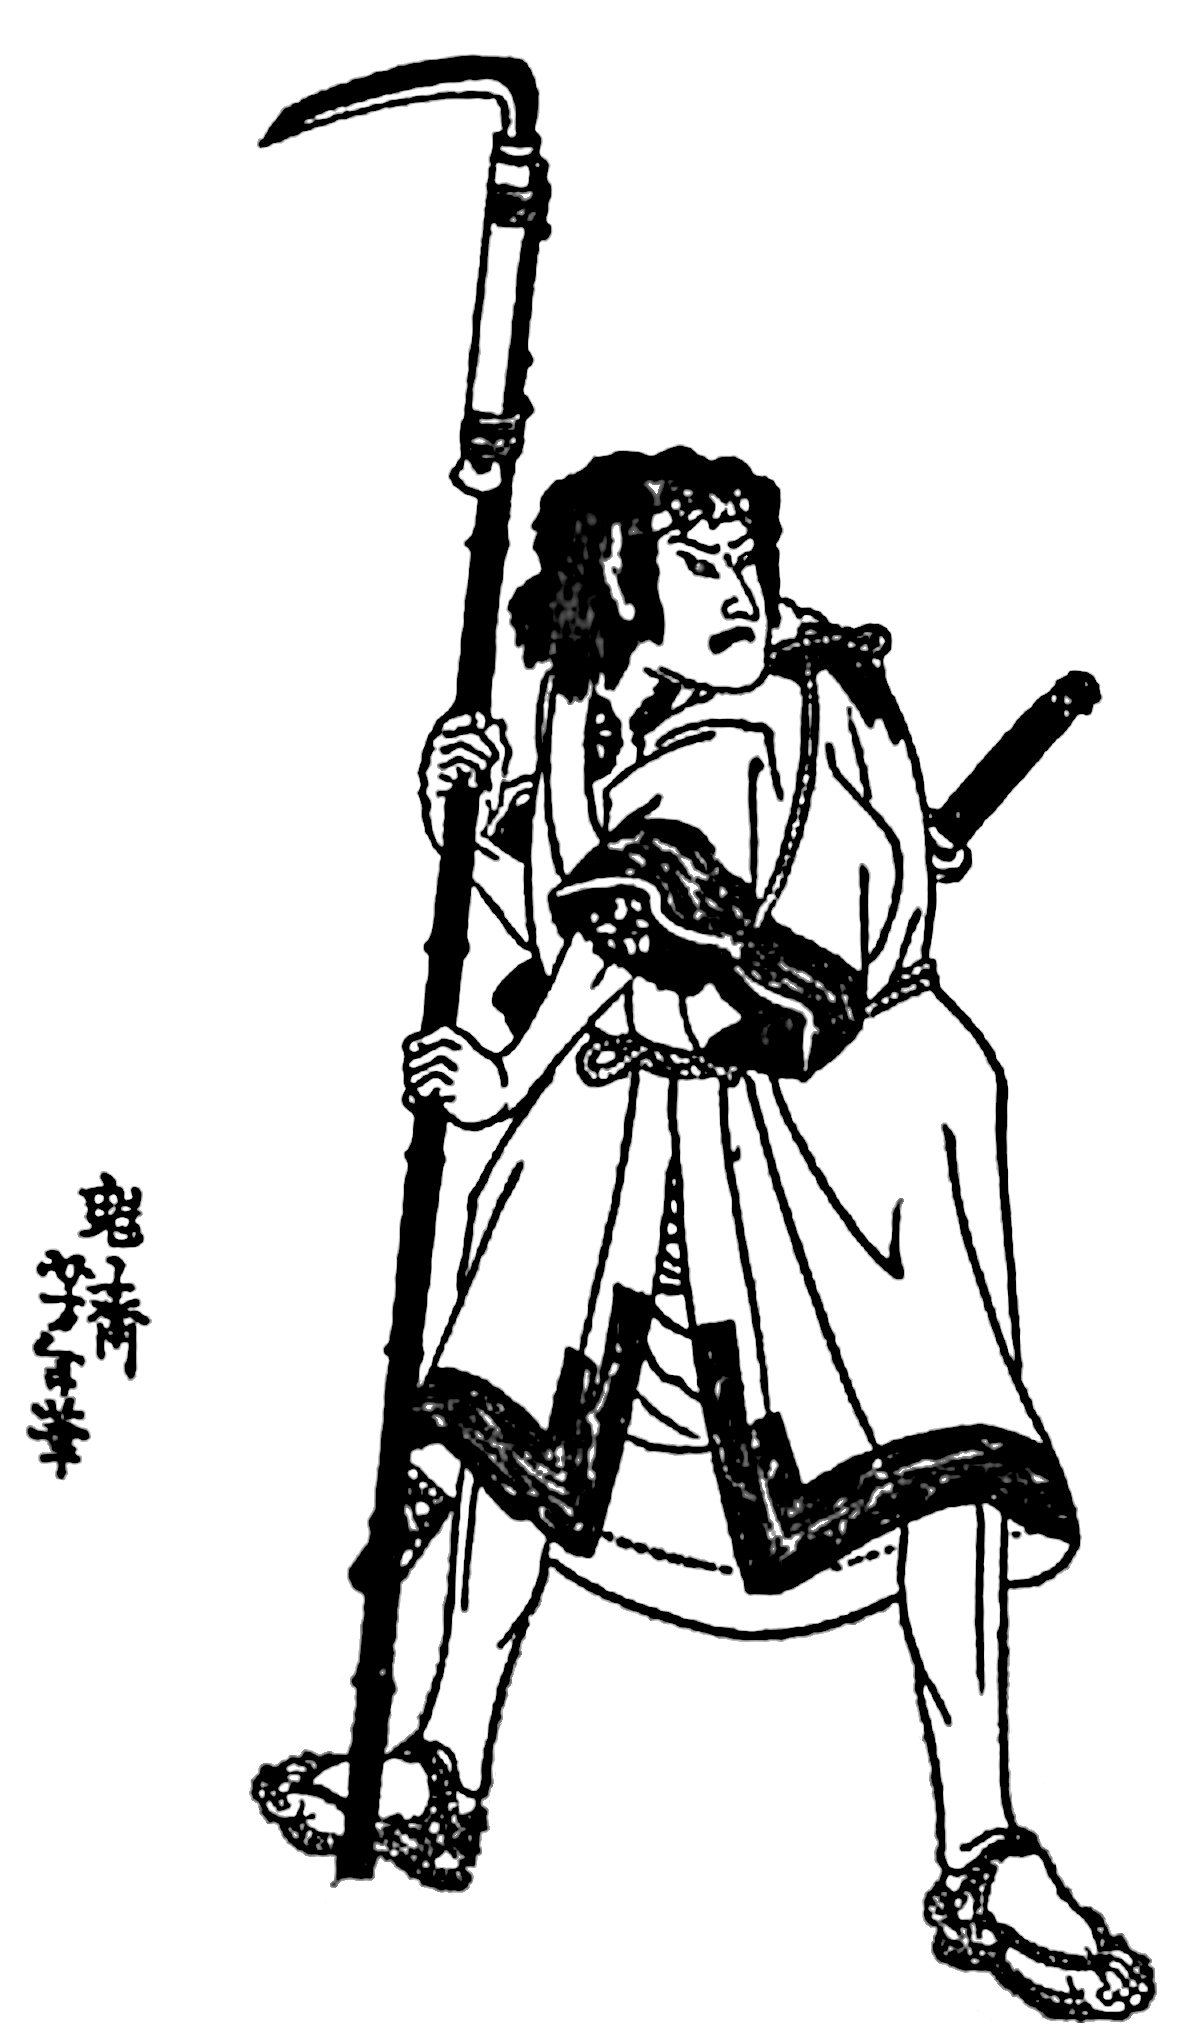
\includegraphics[width=60mm]{naigama}
\end{figure}

\vfill

\begin{table}[]
\centering
\begin{tabular}{ll}
Accompanies release & \input{../../release} \\
Author &  Kees-Jan Hermans / kees.jan.hermans@gmail.com \\
Classification & - \\
Generated on & \today \\
\end{tabular}
\end{table}

% Accompanies release: \input{../../release}
% 
% Author: Kees-Jan Hermans / kees.jan.hermans@gmail.com
% 
% Classification: -
% 
% Generated on: \today
\newpage

\tableofcontents

\setlength{\parindent}{4em}
\setlength{\parskip}{1em}

\newpage
\section{Introduction}

\subsection{Parsing Expression Grammars}

This is the documentation describing gpeg, which is a collection of
specifications, libraries and tools enabling data parsing. It is based, by
now loosely, on Lua Parsing Expression Grammars, or LPEG [REF].

\subsection{gpeg}

gpeg adds to Lua PEG the following features:

\begin{itemize}
\item Discoverability features:

  \begin{itemize}
  \item An assembler step in between grammar and bytecode.
  \item An engine debugger.
  \item A bytecode disassembler.
  \end{itemize}

\item Security features:

  \begin{itemize}
  \item Bit upset event detection and traps.
  \item Endless loop detection.
  \end{itemize}

\item Interoperability with C (library, header files).
\item As well as Java, Perl and Rust.
\item Added instructions for matchers (ranges, quads).
\item Added instructions for counters (to enable efficient looping).
\item Added instructions for parsing binary inputs.
\end{itemize}


\newpage
\section{Overview}

This document describes the gpeg parsing system, which is a 
modular system to process structured arbitrary length data inputs,
in order to extract meaning (matching, capturing from data), or to
manipulate (replacements within data).
The system was designed with a focus on information and system security.

The system comes in three parts: a grammar compiler, an assembler,
and a bytecode execution engine. Each of the parts has their own
input file format specification (grammar description, assembly specification,
and bytecode specification), and outputs the format of the next stage.
The process in brief: the compiler takes a
grammar description that the human user has made, and turns it into
an assembly language. The assembler takes the assembly, and turns it
into a bytecode. The engine takes the bytecode and the input, and
processes it, resulting either in (various measures of) failure or
success.

%\begin{myquote}
%\begin{verbatim}
%Program:      _ Compiler       _  Assembler       _ Engine
%              /|         \     /|           \     /|  /|\  \
%             /           _\|  /             _\|  /     |   _\|
%Format: Grammar          Assembly           Bytecode   |   Output
%                                                       |
%                                                     Input
%\end{verbatim}
%\end{myquote}
%\textit{Schematic overview of gpeg data format transformation and modules}

\begin{center}
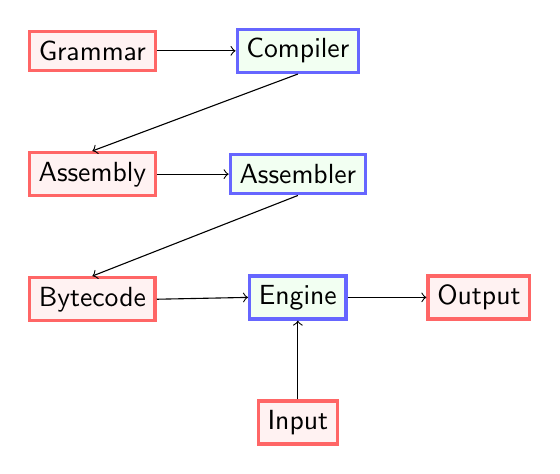
\begin{tikzpicture} [
bluenode/.style={rectangle, draw=blue!60, fill=green!5, very thick, minimum size=5mm},
rednode/.style={rectangle, draw=red!60, fill=red!5, very thick, minimum size=5mm},
]
%Nodes
\node[rednode]     (grammar)                            {Grammar};
\node[bluenode]    (compiler)    [right=of grammar]     {Compiler};
\node[rednode]     (assembly)    [below=of grammar]     {Assembly};
\node[bluenode]    (assembler)   [below=of compiler]    {Assembler};
\node[rednode]     (bytecode)    [below=of assembly]    {Bytecode};
\node[bluenode]    (engine)      [below=of assembler]   {Engine};
\node[rednode]     (input)       [below=of engine]      {Input};
\node[rednode]     (output)      [right=of engine]      {Output};

%Lines
\draw[->] (grammar.east) -- (compiler.west);
\draw[->] (compiler.south) -- (assembly.north);
\draw[->] (assembly.east) -- (assembler.west);
\draw[->] (assembler.south) -- (bytecode.north);
\draw[->] (bytecode.east) -- (engine.west);
\draw[->] (input.north) -- (engine.south);
\draw[->] (engine.east) -- (output.west);

\end{tikzpicture}

\textit{Schematic overview of gpeg transformations: data formats (red) and tools (blue).}

\end{center}


The reason for this modularity is strict separation of tasks, and openness:
anyone should be able to take out a module, and replace it with one
of their own.
It should be expressly possible to take out the compiler, and replace
it with another tool that produces the gpeg assembly, for example.
Or have a different engine. Or write an optimizer for the assembly.

\subsection{On Grammar}
  
gpeg grammar is the human interface of the system.
It can be used to define complex syntax definitions in order
to match, capture from, and replace in, structured inputs.

People familiar with regular expressions \cite{bib:regex},
Backus-Naur syntax descriptions \cite{bib:backusnaur},
and / or Lex and Yacc tools \cite{bib:yacc},
should find this part of the document relatively easy to understand.
The ideas underlying gpeg grammar, assembly and bytecode
are heavily borrowed from Lua PEG (LPEG) \cite{bib:peg}
by Roberto Ierusalimschy et al.

\subsection{On Assembly}

The gpeg assembly language is a mixture of two languages:
For one, it is the outcome instruction set, according to the
aforementioned LPEG whitepaper,
of the gpeg grammar compilation process. However, it also contains
instructions that won't be produced by this compiler, but may
either be produced by a separate optimizer, or other compilers
altogether (for example, one that focuses on network packet
parsing).

The gpeg assembly language, in all cases, is the human readable
variant of the gpeg bytecode, and its instructions are one-on-one
translatable from the one to the other, and vice versa
(although labels will be lost in the reverse process).

\subsection{On Bytecode}

gpeg bytecode is the machine interface of the system.
It runs in the gpeg engine against the input provided by the user.
It is designed to be:

\begin{itemize}

\item Easy and quick to interpret.
\item Resilient against bit upset events.
\item Resilient against endless loops.
\item Usable while keeping both bytecode and input as read-only buffers.

\end{itemize}


\newpage
\section{Generations}

gpeg is written in generations. That is to say:
each subsequent generation of gpeg uses the tools generated
in the previous one, to build itself ('the grammar parses the grammar').

The following generations exist, with the following functions:

\begin{itemize}

\item Generation zero: This generation consists solely of a bootstrap
      grammar compiler and assembler written in perl. Plus a C engine
      to be used by the subsequent generation.

\item Generation one: This generation is
      built in C, based on the bytecode to parse grammar grammar
      and assembly grammar, generated by generation zero.

\item Generation two: equal to generation one, but then based on
      the bytecode generated by the tooling in generation one.
      Generation two is 'pure' in that it has compiled itself,
      and it only provides parsing.

\end{itemize}


\newpage
\section{Grammar}
\label{sec:grammar}

A gpeg grammar file or buffer consists either of a single
unnamed expression, or of a sequence of named expressions (called rules),
whitespace and comments, denoted in ASCII text.
gpeg grammar is defined with the express purpose of matching, validating
and/or capturing from an arbitrary data input.
gpeg grammar is taken by the gpeg compiler program (gpegc) and turned
into gpeg assembly [section \ref{sec:assembly}].
In this, it resembles greatly other grammar description and parsing methods
such as Backus-Naur, Regular Expressions, Lex and Yacc.

\begin{myquote}
\begin{verbatim}
-- JSON; JavaScript Object Notation.
TOP          <- JSON
__prefix     <- %s*
JSON         <- HASH END
HASH         <- CBOPEN OPTHASHELTS CBCLOSE
OPTHASHELTS  <- HASHELTS / ...
HASHELTS     <- HASHELT COMMA HASHELTS / HASHELT
HASHELT      <- STRING COLON VALUE
ARRAY        <- ABOPEN OPTARRAYELTS ABCLOSE
OPTARRAYELTS <- ARRAYELTS / ...
ARRAYELTS    <- VALUE COMMA ARRAYELTS / VALUE
VALUE        <- STRING / FLOAT / INT / BOOL / NULL / HASH / ARRAY
STRING       <- { '"' ( '\\' ([nrtv"] / [0-9]^3) / [^"\\] )* '"' }
INT          <- { [0-9]+ }
FLOAT        <- { [0-9]* '.' [0-9]+ }
BOOL         <- { 'true' / 'false' }
NULL         <- { 'null' }
CBOPEN       <- '{'
CBCLOSE      <- '}'
ABOPEN       <- '['
ABCLOSE      <- ']'
COMMA        <- ','
COLON        <- ':'
END          <- !.
\end{verbatim}
\end{myquote}
\textit{Example of a gpeg grammar meant to validate and capture from
JSON\cite{bib:json} text.}

\subsection{Caveats}

This section highlights a few things to keep in mind when using
gpeg, or PEGs in general.

\subsubsection{Greedy and Blind Behavior}

PEG is, by itself, both greedy and blind.
That is to say, it consumes as much input as possible (greedy), and it does not
look ahead whether a next token is perhaps a better match for the input (blind).
It can however, also implement non-blind behavior, both in a greedy as
well as a non-greedy manner.

Having a greedy, blind parser - standard PEGs - implies that the following
rule will always fail (because the '.*' will consume all input):

\begin{myquote}
\begin{verbatim}
RULE <- .* 'foo'
\end{verbatim}
\end{myquote}

Grammars or patterns like the above, are usually treated in a more
friendly way by, for example, Regex parsers. They implement
a recursive algorithm around 'does the whole pattern match' question,
which backtracks 'from zero to any amount' quantifiers such as the one
used above,
leaving the user with a much more freedom to implement patterns but,
in the end, a much more unpredictable system (for example, what if
'foo' happens twice in the text?)

gpeg is not so understanding. To make it match something while
also doing a lookahead (therefore 'non blind'),
you can implement the following pattern
recursively (non greedy, so catching the first lookahead match):

\begin{myquote}
\begin{verbatim}
S <- E2 / E1 S
\end{verbatim}
\end{myquote}

Or, not recursively:

\begin{myquote}
\begin{verbatim}
S <- ( !E2 E1 )* E2
\end{verbatim}
\end{myquote}

And greedy, so catching only the last lookahead match:

\begin{myquote}
\begin{verbatim}
S <- E1 S / E2
\end{verbatim}
\end{myquote}

\subsubsection{Recursiveness}

Just like with greedy matching, gpeg will simply jump headlong
into your rule's first matcher, and will not try to second-guess your
intentions. So while in many grammar systems, left recursive is
usually considered the best way to describe
repetition, PEG will get stuck in an endless loop if you do the following:

\begin{myquote}
\begin{verbatim}
S <- S SOMEOTHER
\end{verbatim}
\end{myquote}

\subsection{Comments}

A comment starts with two minus signs and ends at the end of the line.

\begin{myquote}
\begin{verbatim}
-- Example of a single line comment.
\end{verbatim}
\end{myquote}

A multiline comment is also avaiable: these start with two minus signs
followed by two angle braces. The multiline comment is closed by two
closing angle braces.

\begin{myquote}
\begin{verbatim}
--[[
     Example of a
     multiline comment.
  ]]
\end{verbatim}
\end{myquote}

\subsection{Rules}

A rule is defined as an \textit{Identifier}, followed by a
left-pointing arrow (composed of a less-than and a minus sign),
followed by a matching expression.

When a gpeg grammar consists of a sequence of rules
(as opposed to a single line expression),
the first rule is used as the starting point for matching inputs.

\begin{myquote}
\begin{verbatim}
RULE1 <- 'a' / RULE2
RULE2 <- 'b' / RULE3
RULE3 <- 'c'
\end{verbatim}
\end{myquote}
\textit{Definition of a set of rules}

\subsubsection{Identifiers}

Identifiers, in gpeg, are defined as a combination of letters,
numbers and the underscore character, not starting with a number,
of between one and 64 characters long.

\begin{myquote}
\begin{verbatim}
IDENTIFIER <- [a-zA-Z_][a-zA-Z0-9_]^-63
\end{verbatim}
\end{myquote}

Identifiers are used to start rule definitions, and as references
to rules in expressions.

\subsubsection{Special Rules}

There is currently one special rule in gpeg grammar: a rule called
'\_\_prefix' will be treated specially. This rule will be, from its
definition onwards, called before the execution of any subsequent rule
definition expression. The aim is to make whitespace and comment filtering
in program language parsing easier. See also the earlier 'JSON' grammar
example.

\subsection{Expressions}

Expressions are lists of terms, optionally separated by the
OR operator (denoted by the forward slash sign).

\begin{myquote}
\begin{verbatim}
ALTERNATIVES <- ALT1 / ALT2 / ALT3
\end{verbatim}
\end{myquote}

A sequence of terms has a higher precendence than the OR operator,
so any other desired order of precedence has to be forced by using
brackets.
In the example below, the expressions evaluate differently:

\begin{myquote}
\begin{verbatim}
RULE1 <- 'a' 'b' / 'c'
RULE2 <- 'a' ( 'b' / 'c' )
\end{verbatim}
\end{myquote}

\subsection{Terms}

A term is defined as a matcher, potentially adorned with prefix
or postfix operators (though not at the same time).
Prefix operators are the NOT and CONFIRM modifiers.
Postfix operators are the quantifiers.

\subsubsection{The NOT Modifier}

The NOT modifier is an exclamation mark.
It does not advance the input position, but succeeds
when matching fails (including reaching the end of input),
and fails when matching succeeds.
Since gpeg is a greedy parser,
this can be used to implement a non-greedy lookahead, for example:
 
\begin{myquote}
\begin{verbatim}
CMULTILINECOMMENT <- '/*' (!'*/' .)* '*/'
\end{verbatim}
\end{myquote}

\subsubsection{The CONFIRM Modifier}

The CONFIRM modifier is an ampersand.
It does not advance the input position, and succeeds
as matching succeeds, and fails when matching fails.
It can be used to process (parts of the) input twice.
It is equivalent to using the NOT modifier twice.

Example where the input is first confirmed to be valid UTF-8,
and only after that, processed again from the beginning, for
well-formedness.
\begin{myquote}
\begin{verbatim}
JSON <- & UTF8 WELLFORMED
\end{verbatim}
\end{myquote}

\subsubsection{Quantifiers}

gpeg denotes quantifiers using a circonflex, followed by either
an absolute number, or a range. Shorthand exists for certain, often-used
ranges. These shorthand ranges are common in Regex as well:

\begin{center}
%\caption{gpeg Quantifiers}
\label{tab:naig_quantifiers}
\begin{longtable}{ll}
\textbf{Quantifier} & \textbf{Semantics} \\
\endhead
* & Zero or more matches \\
+ & One or more matches \\
? & Zero or one matches \\
\^{}\textit{n} & \textit{n} matches \\
\^{}-\textit{n} & Zero up to and including \textit{n} matches \\
\^{}\textit{n}- & \textit{n} matches or more \\
\^{}\textit{n}-\textit{m} & From \textit{n} up to and including \textit{m} matches \\
\end{longtable}
\end{center}
 
Example of the use of quantifiers:
\begin{myquote}
\begin{verbatim}
RULE1 <- 'a'? 'b'^-5
\end{verbatim}
\end{myquote}

\subsection{Matchers}

\subsubsection{The ANY Matcher}

The ANY matcher is denoted (like in Regex) with a single dot.
It matches any character of input and it succeeds - advancing the input
pointer by one - if it can find one at the input pointer. It fails only
at the end of input.

\begin{myquote}
\begin{verbatim}
RUNGREEDILYTOTHEENDOFINPUT <- .*
\end{verbatim}
\end{myquote}

\subsubsection{The SET Matcher}

The ANY matcher, together with the NOT modifier,
also allows you to define end-of-input, like so:

\begin{myquote}
\begin{verbatim}
ENDOFINPUT <- !.
\end{verbatim}
\end{myquote}

\subsubsection{The SET Matcher}

The SET matcher is denoted, like in Regex, as a series of literals
and ranges, enclosed between angled brackets. It can also be negated,
in which case it matches any character not in the set.

\begin{myquote}
\begin{verbatim}
ALPHABETIC     <- [a-zA-Z]
NONALPHABETIC  <- [^a-zA-Z]
\end{verbatim}
\end{myquote}

The denotation of the set elements has a backslash as escape character
(to encode the minus and the closing angled brace).
It also has a form of binary escaping, to encode non-ASCII characters
as part of the set: a backslash followed by three digits of the characters
octal notation.

\subsubsection{The STRING Matcher}

The STRING matcher is denoted as a string literal, between single
quotes. The string may be postfixed with an lower case 'i' to
indicate (alphabetic) case insensitive matching.

\begin{myquote}
\begin{verbatim}
CASEINSENSTIVESTRING <- 'peg'i
\end{verbatim}
\end{myquote}

\subsubsection{The BITMASK Matcher}

The BITMASK matcher allows you to match bits.

\subsubsection{The HEXLITERAL Matcher}

The HEXLITERAL matcher allows you to match single characters by
through their hexadecimal representation.

\subsubsection{The MACRO Matcher}

All macroes are shorthand equivalents of the SET matcher.

\begin{center}
%\caption{gpeg Macroes}
\label{tab:naig_macroes}
\begin{longtable}{lll}
\textbf{Macro} & \textbf{Semantics} & \textbf{Set} \\
\endhead
\%s & Whitespace & [ \textbackslash n\textbackslash r\textbackslash t\textbackslash v] \\
\%w & Alphabetic & [a-zA-Z] \\
\%a & Alphanumeric & [a-zA-Z0-9] \\
\%n & Numeric & [0-9] \\
\%p & Printable & 0x20 - 0x7f \\
\end{longtable}
\end{center}

\subsubsection{The GROUP Matcher}

\subsubsection{The CAPTURE Matcher}

\subsubsection{The VARCAPTURE Matcher}

\subsubsection{The VARREFERENCE Matcher}

\subsubsection{The REFERENCE Matcher}

\subsubsection{The LIMITEDINPUT Matcher}

\subsubsection{The END Matcher}



\newpage
\section{Compilation}

This section deals with the more holistic side of the compilation process,
which transforms grammar into assembly.

\subsection{Named or Anonymous Grammars}

gpeg allows two types of grammars:

\begin{itemize}
\item Named grammars, which consist of a list of named rules.
\item Anonymous grammars, which consist of a single expression.
\end{itemize}

\subsection{Imports}

Imports are treated more or less in the way that C treats '\#include's:
file contents are substituted in place, and re-evaluated. The caveat
is that this must happen at rule definition level: you cannot have
substitutions of file contents, for example, in a sequence of matchers,
or as part of a matcher (for example, inside a string).

Other caveats to the import function are: a limit to the amount of
recursion allowed, and all importing happens in the same namespace
(therefore, any recursion should result in a namespace clash error
anyway).

\subsection{Special Keywords}

\subsubsection{The '\_\_prefix' Rule}

The \_\_prefix rule will define a pattern that is called before
the evaluation of every rule that follows it. This is typically
done to remove things like whitespace and comments while parsing
things like source code or text based data formats (XML, JSON, etc).

\subsubsection{The '\_\_main' Rule}

The '\_\_main' rule, which does not have to be defined, but if it is,
it will be called first. This may be convenient when the \_\_prefix and
first rule to be called cause a grammar rule topological conflict.

\subsubsection{The '\_\_end' Matcher}

The '\_\_end' matcher, which is not a matcher but actually more like
inline assembly, is nevertheless defined part of a sequence
of matchers. It successfully ends execution of the bytecode.
The compiler simply inserts an 'end' assembly instruction at that point.

\subsection{Determining the First Rule}

A named grammar will call as the first rule:

\begin{itemize}
\item The rule called '\_\_main', or in absence of such a rule:
\item The first defined rule.
\end{itemize}

The compiler will emit a 'call' instruction to the first rule as the
first instruction, followed by an 'end' instruction ('end 0').


\newpage
\section{Assembly}
\label{sec:assembly}

A gpeg assembly file or buffer consists of sequences of
whitespace, comments, labels, and (parametrized) instructions, separated
by new lines, and denoted in ASCII text.

gpeg assembly is taken by the gpeg assembler program (naia) and turned
into bytecode.

\begin{myquote}
\begin{verbatim}
-- Compilation of: TEST <- { 'a' } { 'a' } { 'a' / 'b' }
  call TEST
  end
-- Rule
TEST:
  opencapture 0
  char 61
  closecapture 0 0
  opencapture 1
  char 61
  closecapture 1 0
  opencapture 2
  catch __LABEL_30 -- alternative
  char 61
  commit __LABEL_31
__LABEL_30:
  char 62
__LABEL_31:
  closecapture 2 0
  ret
\end{verbatim}
\end{myquote}
\textit{Example of a piece of gpeg assembly}

\subsection{Comments}

Just like in gpeg grammar,
comments in gpeg assembly start with two minus signs, and end at
a new line. They can be given on separate lines, or they can be
postfixed to instructions or labels.

\subsection{Labels}

Labels are identifiers (the same identifiers as in their definition
in the grammar chapter) or numbers, followed by a colon sign. They are used
as positions for the bytecode to jump to, when used by instructions.

When performing the assembly, the gpeg assembler program resolves
each label to their offset in the resultant bytecode, and replaces each
reference to a label with that offset.

Labels don't quite disappear though - you have the option to make the
assembler program emit a so called 'labelmap' file, which stores the old
label names, mapped to the bytecode offsets given by the assembler,
and which can be used later
for debugging purposes by the bytecode execution engine.

When disassembling (bytecode to assembly), each instruction is always
prefixed by a label in the form of the instruction's offset in decimal,
so that jumps are always correct (but non descriptive).

\subsubsection{Special Labels}

Certain instructions allow a special label called '\_\_NEXT\_\_' to be
used as parameter. Its function is to make instruction simply jump to
the next instruction on success.
This special label is there to avoid generating a special purpose label
only to put it right after the instruction using it.

The instructions allowing the use of the '\_\_NEXT\_\_' label are:

\begin{itemize}
\item backcommit
\item commit
\item condjump
\item partialcommit
\item testany
\item testchar
\item testquad
\item testset
\end{itemize}

\subsection{Instructions}


%\begin{table}[]
\begin{center}
%\caption{gpeg Assembly Instructions}
\label{tab:naig_assembly}
\begin{longtable}{lll}
\textbf{Mnemonic} & \textbf{Param1} & \textbf{Param2} \\
\endhead
'any' &  &  \\
'backcommit' &  & LABEL \\
'bitmask' & nbits & bits \\
'call' &  & LABEL \\
'catch' &  & LABEL \\
'char' & char &  \\
'closecapture' & slot &  \\
'commit' &  & LABEL \\
'condjump' & register & LABEL \\
'counter' & register & value \\
'end' & code &  \\
'endisolate' &  &  \\
'endreplace' &  &  \\
'fail' &  &  \\
'failtwice' &  &  \\
'intrpcapture' &  &  \\
'isolate' & slot &  \\
'jump' &  & LABEL \\
'noop' &  &  \\
'opencapture' & slot &  \\
'partialcommit' &  & LABEL \\
'quad' & quad &  \\
'range' & from & until \\
'replace' & slot & LABEL \\
'ret' &  &  \\
'set' & set &  \\
'skip' & number &  \\
'span' & set &  \\
'testany' &  & LABEL \\
'testchar' & char & LABEL \\
'testquad' & quad & LABEL \\
'testset' & set & LABEL \\
'trap' &  &  \\
'var' & slot &  \\
\end{longtable}
\end{center}
%\end{table}


See table [\ref{tab:naig_assembly}].

\subsection{Parameters}

Parameters follow the instruction in assembly text. They are separated
from the instruction and any other parameters by spaces. The following
types of parameters exist:

\subsubsection{Characters}

Character parameters are denoted as two byte hexadecimal values.

\subsubsection{Quads}

Quad parameters are denoted as eight byte hexadecimal values.

\subsubsection{Sets}

Set parameters are denoted as 64 byte hexadecimal values, representing
a bitmask of 256 possible booleans.

\subsubsection{Registers, Slots, Codes and Numbers}

These parameters are all denoted as decimal numbers.

\subsubsection{Caveats}

Note that the order of parameters sometimes reverses between the assembly
and bytecode specification. This is done because in assembly, it is
considered more aesthetically pleasing to have labels at the end of an
instruction, while in bytecode they are usually given as the first argument.

Consider, for example, the 'testchar' instruction, which in assembly is
given as:

\begin{myquote}
\begin{verbatim}
TESTCHARINSTR <- { 'testchar' } S HEXBYTE S LABEL
S <- %s+
HEXBYTE <- { [0-9a-fA-F]^2 }
LABEL <- { [a-zA-Z0-9_]^1-256 }
AMPERSAND <- '&'
\end{verbatim}
\end{myquote}

Whereas in bytecode, this instruction is encoded as:

%DEADBEEF
$_{00}$\ 
\fbox{%
  \parbox{20pt}{%
00
  }%
}
\fbox{%
  \parbox{20pt}{%
08
  }%
}
\fbox{%
  \parbox{20pt}{%
03
  }%
}
\fbox{%
  \parbox{20pt}{%
9a
  }%
}



$_{04}$\ 
\fbox{%
  \parbox{20pt}{%
00
  }%
}
\fbox{%
  \parbox{20pt}{%
00
  }%
}
\fbox{%
  \parbox{20pt}{%
00
  }%
}
\fbox{%
  \parbox{20pt}{%
00
  }%
}



$_{08}$\ 
\fbox{%
  \parbox{20pt}{%
00
  }%
}
\fbox{%
  \parbox{20pt}{%
00
  }%
}
\fbox{%
  \parbox{20pt}{%
00
  }%
}
\fbox{%
  \parbox{20pt}{%
00
  }%
}

Where:
  
Bytes 0-3 denote the instruction opcode.

Bytes 4-7 denote the bytecode offset to jump to, after
this instruction (big endian 32 bit unsigned).

Bytes 8-11 denote the character to match.


\newpage
\section{Optimizations}

A PEG compiler only needs to be able to emit the following instructions to be
functionally complete:

\begin{itemize}
\item any
\item backcommit
\item call
\item char
\item closecapture
\item commit
\item end
\item fail
\item failtwice
\item intrpcapture
\item maskedchar
\item opencapture
\item partialcommit
\item ret
\item set
\item var
\end{itemize}

And even about this set, a discussion is possible:
Because theoretically, the 'char' and 'any' instructions are implied by
the 'set' instruction
(although that would bring with it a lot of bytecode overhead).
Also, 'intrpcapture', 'maskedchar' are specific to gpeg and
binary parsing.

Nevertheless, it's sometimes easy and efficient (both from a bytecode
size and execution speed perspective) to optimize the code somewhat.
Which is why the gpeg instruction set is somewhat bigger than the
list above.

\subsection{Optimizing Loops}
A matcher that is quantified for a range can be written out in
full, but gpeg introduces a set of counter registers for this operation,
as well as two instructions to use them: 'counter' and 'condjump'.
Grammar:

\begin{myquote}
\begin{verbatim}
'a'^3
\end{verbatim}
\end{myquote}

Is formally compiled to:

\begin{myquote}
\begin{verbatim}
  char 61
  char 61
  char 61
\end{verbatim}
\end{myquote}

And will be optimized in gpeg as:

\begin{myquote}
\begin{verbatim}
  counter 0 3
looplabel:
  char 61
  condjump 0 looplabel
\end{verbatim}
\end{myquote}

This optimization starts to make a lot more sense when the matcher
is quantified with values much higher than three. Which is why
gpeg performs this optimization automatically.

\subsection{Optimizing Sequences of Char}

gpeg has an instruction to match four bytes at once, called 'quad'.
To optimize matching larger string literals, these are chopped up into
chunks of four bytes, which each emit a 'quad' instruction,
and the remainder is emitted as char instructions.
Grammar:

\begin{myquote}
\begin{verbatim}
'gpeg'
\end{verbatim}
\end{myquote}

Is compiled to:

\begin{myquote}
\begin{verbatim}
  char 4e
  char 61
  char 69
  char 67
  char 61
  char 6d
  char 61
\end{verbatim}
\end{myquote}

May be optimized as:

\begin{myquote}
\begin{verbatim}
  quad 4e616967
  char 61
  char 6d
  char 61
\end{verbatim}
\end{myquote}

\subsection{Optimizing Sets}
When a set consists of a single range, it can be rewritten as a 'range'
instruction.

\begin{myquote}
\begin{verbatim}
[a-z]
\end{verbatim}
\end{myquote}

Compiles to:

\begin{myquote}
\begin{verbatim}
  set 000000000000000000000000feffff0700000000000000000000000000000000
\end{verbatim}
\end{myquote}

May be optimized as:

\begin{myquote}
\begin{verbatim}
  range 97 122
\end{verbatim}
\end{myquote}

\subsection{Optimizing Unlimited Sets}

Span

\subsection{Optimizing Dot-Quantified}

Skip

\subsection{Optimizing Tests}


\newpage
\section{Bytecode}
\label{sec:bytecode}

\subsection{Instruction sets}

gpeg, generation 3, provides two instruction sets (with a few overlapping
instructions) that each have their own stack and other memories:
one for matching, and one for script execution.


%\begin{table}[]
\begin{center}
%\caption{gpeg Bytecode Instructions}
\label{tab:naig_bytecode}
\begin{longtable}{lllll}
\textbf{Mnemonic} & \textbf{Opcode} & \textbf{Param1} & \textbf{Param2} & \textbf{Length} \\
\endhead
any & 000003e4 &  &   & 4 \\
backcommit & 000403c0 & address &   & 8 \\
bitmask & 00100365 & nbits & bits  & 20 \\
call & 00040382 & address &   & 8 \\
catch & 00040393 & address &   & 8 \\
char & 000403d7 & char &   & 8 \\
closecapture & 00040300 & slot &   & 8 \\
commit & 00040336 & address &   & 8 \\
condjump & 00080321 & register & address  & 12 \\
counter & 00080356 & register & value  & 12 \\
end & 000400d8 & code &   & 8 \\
fail & 0000034b &  &   & 4 \\
failtwice & 00000390 &  &   & 4 \\
intrpcapture & 0008000f &  &   & 12 \\
jump & 00040333 & address &   & 8 \\
noop & 00000000 &  &   & 4 \\
opencapture & 0004039c & slot &   & 8 \\
partialcommit & 000403b4 & address &   & 8 \\
quad & 0004037e & quad &   & 8 \\
range & 000803bd & from & until  & 12 \\
ret & 000003a0 &  &   & 4 \\
set & 002003ca & set &   & 36 \\
skip & 00040330 & number &   & 8 \\
span & 002003e1 & set &   & 36 \\
testany & 00040306 & address &   & 8 \\
testchar & 0008039a & address & char  & 12 \\
testquad & 000803db & address & quad  & 12 \\
testset & 00240363 & address & set  & 40 \\
trap & ff00ffff &  &   & 4 \\
var & 000403ee & slot &   & 8 \\
\end{longtable}
\end{center}
%\end{table}


\subsection{Bytecode Structure}

A gpeg bytecode file or buffer consists of a sequence of binary
instructions which, in turn, each consist of a binary
encoded opcode, plus their parameters, should they have any.

The amount and kind of parameters following an opcode, is strictly
defined:
the same opcode will always be followed by the same kinds of parameters
and therefore, an instruction type will always be the same size
(see table [\ref{tab:naig_bytecode}]).

gpeg bytecode is taken by the gpeg engine program (naie) or
library, and run against an input, to produce an output.

\subsection{Opcode Values}

Opcode values are determined through

\begin{itemize}
\item Grouping; 
\item Hamming distance;
\item Instruction size;
\end{itemize}

\subsection{Noop Slides and Canaries}

Implementations that want each instruction to have exactly the
same size, can choose to pad the encoding of shorter instructions
with either no-ops, or canaries.

\subsection{Encoding of Parameters}

\subsubsection{Address}

\subsubsection{Char}

\subsubsection{Slot}

\subsubsection{Register}


\newpage
\section{Output}

When the gpeg engine exits, it may do so in the following states:

\begin{itemize}
\item Engine failure. The engine got corrupted somehow. This is not
      recoverable. You should restart any relevant software in this case.
\item Bytecode failure. The bytecode caused an endless loop, tried
      to jump to an out-of-bounds offset, or contained an unknown
      instruction opcode.
\item Parsing failure. The stack was unwound without seeing the 'end'
      instruction first. Your input does not match your grammar.
\item Parsing success. The engine encountered an 'end' instruction.
      Your input matches your grammar.
\item Parsing success including captures.
      The endine encountered an 'end' instruction and there where
      captures.
\end{itemize}

[TBW]

\subsection{Language Agnostic Output}

The language agnostic way in which gpeg provides output, is a table.
This table is structured as follows:

[TBW]

\subsection{API Outputs}

[TBW]


\newpage
\section{Executables}
\label{exe:main}

\subsection{The Compiler}
\label{exe:gpegc}

The gpeg grammar compiler is called 'gpegc'.
It takes a grammar file as input, and outputs assembly text.
It can be invoked as follows:

\begin{myquote}
\begin{verbatim}
$ gpegc -i myfile.niag -o myfile.asm
\end{verbatim}
\end{myquote}
\textit{Example of the invocation of the gpeg grammar compiler}

Bear in mind that both the input (grammar) file, as well as the
output (assembly) file may be omitted (in which case they will be
assumed to be stdin and stdout, respectively), or be denoted as
a minus sign ('-'), which will have the same effect.

You may also use the following options:

\begin{itemize}
\item \texttt{-m $<$path$>$} Tells the compiler to emit the slotmap
      file in $<$path$>$.
\item \texttt{-D} Creates a lot of debugging output.
\item \texttt{-t} Tells the compiler to surround generated rule
      code with 'trap' instructions.
\end{itemize}

\subsection{The Assembler}
\label{exe:gpega}

The gpeg grammar assember is called 'gpega'.
It takes an assembly file as input, and outputs bytecode.
It can be invoked as follows:

\begin{myquote}
\begin{verbatim}
$ gpega -i myfile.asm -o myfile.byc
\end{verbatim}
\end{myquote}
\textit{Example of the invocation of the gpeg assembler}

Bear in mind that both the input (assembly) file, as well as the
output (bytecode) file may be omitted (in which case they will be
assumed to be stdin and stdout, respectively), or be denoted as
a minus sign ('-'), which will have the same effect.

You may also use the following options:

\begin{itemize}
\item \texttt{-l $<$path$>$} Tells the assembler to emit the labelmap
      file in $<$path$>$.
\item \texttt{-D} Creates a lot of debugging output.
\end{itemize}

\subsection{The Engine}

The gpeg bytecode execution engine is called 'gpege'.
It takes a bytecode file as input, as well as an input file.
It can be invoked as follows:

\begin{myquote}
\begin{verbatim}
$ gpege -c myfile.byc -i myfile.dat -o myfile.out
\end{verbatim}
\end{myquote}
\textit{Example of the invocation of the gpeg engine}

\subsection{The Disassembler}

The gpeg disassembler is called 'gpegd'.
It takes a bytecode file as input, and outputs assembly.

\begin{myquote}
\begin{verbatim}
$ gpegd -i myfile.byc -o myfile.asm
\end{verbatim}
\end{myquote}
\textit{Example of the invocation of the gpeg disassembler}

The output of the disassembler will differ from the assembly
generated by the compiler in that:

\begin{itemize}
\item Textual labels will be gone, instead:
\item Every instruction will be prefixed by a numeric label which
      is identical to that instruction's position offset in the bytecode, and
\item All jumps will therefore also be using those position labels.
\end{itemize}


\newpage
\section{File Formats}

This section describes all the user available memory and file formats
associated with gpeg.

\subsection{Grammar}

The gpeg grammar text format is descibed in [\ref{sec:grammar}].
Various pre-compilers can potentially produce these format however,
these are out of scope of this documentation. The grammar format is
consumed by the gpeg assembler, gpegc. For the use of gpegc, see
[\ref{exe:gpegc}].

\subsection{Assembly}

The gpeg assembly text format is descibed in [\ref{sec:assembly}].
This format is produced by the gpeg compiler, gpegc,
and is consumed by the gpeg assembler, gpega.
For the use of gpega, see [\ref{exe:gpega}].

\subsection{Maps}

\subsection{Slotmap.h}

The gpeg compiler assigns a slot number to each capture it encounters.
It then assigns an internal unique name to those capture numbers, or slots.
Finally, the compiler can be requested, through the command line, to
'rain down' these named mappings to slot number in a C-header file, so that
API users can use easy-to-remember \#defines to address their captures.

\subsection{Disassembly}

The gpeg disassembler, naid, will take bytecode and reproduce the
assembly. This assembly will be different from the original assembly
in that:

\begin{itemize}
\item It will not contain textually understandable labels.
\item It will prefix every instruction with a numeric label, which is
      equivalent to the bytecode offset of the instruction's opcode.
\item These offsets will then also be used in jumps.
\end{itemize}

\subsection{Engine Debug Logs}

Running the gpeg engine, naie, in debug mode will yield, on standard error,
a log, which will contain, per instruction executed, a line representing
the engine's internal state, most notably its stack, like so:

\begin{myquote}
\begin{verbatim}
CHAR bc 2316 in 482 0403020100______ st (014 prec.) ALT:1484
CLL:1476 C LL:1820 ALT:1944 CLL:1928 ALT:1652 CLL:1644 CLL:2440
\end{verbatim}
\end{myquote}

These lines are built up as follows:

\begin{itemize}
\item The instruction being executed (in this case, 'char').
\item The bytecode offset (in this case, 2316 decimal).
\item The input offset (in this case, 482 decimal).
\item A subset of the input, from the input offset (in this in hexadecimal).
\item An overview of the stack (in this case, with 14 preceding items left
      out), followed by the last stack items, either 'call' items
      (with their return addresses), or 'alternative' items
      (with their jump-to addresses in case they catch a FAIL condition).
\end{itemize}

This section describes the formats used by the gpeg tooling, other than
the ones described in the sections on grammar, assembly and bytecode.

\subsection{Slotmap Format}

The slotmap file exists to help developers by easing access to
captures in complex grammars.

The gpeg grammar compiler can be instructed to emit a slotmap file.
This is a file which maps a unique name to a capture region's index.
This is provided so that, instead of using the index of capture region
(which requires hand counting them in your grammar file, which can be
tedious and error-prone, and something that would not survive
a grammar reshuffle, or the introduction of a capture region before
the one you're interested in), you can use a naming scheme for your
capture regions.

Names in the slotmap file are bound semantically to the capture region:
they are made up of the name of the rule,
an underscore, and all alphabetic characters in the capture region,
cast to uppercase. Should any name occur twice, it will be postfixed with
a counter until it's unique.

For example, the following rule with capture region definition:

\begin{myquote}
\begin{verbatim}
RULE <- { IDENT } OPTARGS LEFTARROW EXPRESSION
\end{verbatim}
\end{myquote}

will result in slotmap identifier 'RULE\_IDENT'.

The binary format of a slotmap file is composed as a sequence of binary records:
the slot index, denoted as a 32 bit network order unsigned integer, a
field of 32 bit all ones, and the slot name, denoted as a zero-terminated
string.

\begin{myquote}
\begin{verbatim}
00 00 00 00 ff ff ff ff 52 55 4c 45 5f 49 44 45  ........RULE_IDE
4e 54 00 00 00 00 01 ff ff ff ff 45 58 50 52 45  NT.........EXPRE
53 53 49 4f 4e 5f 54 45 52 4d 53 00 00 00 00 02  SSION_TERMS.....
ff ff ff ff 45 58 50 52 45 53 53 49 4f 4e 5f 54  ....EXPRESSION_T
45 52 4d 53 5f 31 00 00 00 00 03 ff ff ff ff 45  ERMS_1.........E
58 50 52 45 53 53 49 4f 4e 5f 54 45 52 4d 53 5f  XPRESSION_TERMS_
32 00 00 00 00 04 ff ff ff ff 54 45 52 4d 53 5f  2.........TERMS_
54 45 52 4d 00 00 00 00 05 ff ff ff ff 54 45 52  TERM.........TER
4d 5f 4e 4f 54 41 4e 44 00 00 00 00 06 ff ff ff  M_NOTAND........
\end{verbatim}
\end{myquote}
\textit{Example of the head of a slotmap file, hex dumped}

\subsection{Labelmap Format}

The labelmap format is optionally emitted by the assembler, and exists to:

\begin{itemize}
\item Allow for better debugging, because offsets in bytecode can be reduced
      to more intuitively named sections (rule names always make it to
      the labelmap unchanged).
\item Allow for calling the bytecode at symbols directly, which in turn
      allows you to use a bytecode blob more as a database of functions.
\end{itemize}

The binary format of the labelmap file is composed as a sequence of
binary records: the bytecode offset, denoted as a 32 bit network order
unsigned integer, followed by the labelstring, followed by a zero byte.

\begin{myquote}
\begin{verbatim}
00 00 00 10 47 52 41 4d 4d 41 52 00 00 00 00 28  ....GRAMMAR....(
5f 5f 4c 41 42 45 4c 5f 31 31 00 00 00 00 38 5f  __LABEL_11....8_
5f 4c 41 42 45 4c 5f 31 32 00 00 00 00 40 5f 5f  _LABEL_12....@__
4c 41 42 45 4c 5f 36 00 00 00 00 48 5f 5f 4c 41  LABEL_6....H__LA
42 45 4c 5f 37 00 00 00 00 54 5f 5f 70 72 65 66  BEL_7....T__pref
69 78 00 00 00 00 5c 5f 5f 4c 41 42 45 4c 5f 32  ix....\__LABEL_2
39 00 00 00 00 7c 5f 5f 4c 41 42 45 4c 5f 34 33  9....|__LABEL_43
00 00 00 00 a8 5f 5f 4c 41 42 45 4c 5f 34 34 00  .....__LABEL_44.
00 00 00 b8 5f 5f 4c 41 42 45 4c 5f 33 32 00 00  ....__LABEL_32..
00 00 e4 5f 5f 4c 41 42 45 4c 5f 35 35 00 00 00  ...__LABEL_55...
01 10 5f 5f 4c 41 42 45 4c 5f 35 36 00 00 00 01  ..__LABEL_56....
10 5f 5f 4c 41 42 45 4c 5f 33 33 00 00 00 01 18  .__LABEL_33.....
5f 5f 4c 41 42 45 4c 5f 33 30 00 00 00 01 1c 45  __LABEL_30.....E
4e 44 00 00 00 01 34 5f 5f 4c 41 42 45 4c 5f 35  ND....4__LABEL_5
38 00 00 00 01 38 44 45 46 49 4e 49 54 49 4f 4e  8....8DEFINITION
00 00 00 01 4c 53 49 4e 47 4c 45 5f 45 58 50 52  ....LSINGLE_EXPR
45 53 53 49 4f 4e 00 00 00 01 60 52 55 4c 45 00  ESSION....`RULE.
00 00 01 a0 45 58 50 52 45 53 53 49 4f 4e 00 00  ....EXPRESSION..
00 01 e4 5f 5f 4c 41 42 45 4c 5f 31 30 36 00 00  ...__LABEL_106..
\end{verbatim}
\end{myquote}
\textit{Example of a section of labelmap file, hex dumped}

\subsection{Engine Output Format}

The gpeg bytecode execution engine, naie, produces, on success, output for
digital processing, in the form of a binary table, which is structured
as follows:

\begin{itemize}

\item Each record is four 32 bit integers, in network order.

\item The first record contains the end code of the matching process.
This is the same code as was given as a parameter to the 'end'
instruction that resulted in the execution finishing. This is the
first field, by default it is zero.
The second field contains the amount of subsequent records.

\item Subsequent records have as fields, either:

\begin{itemize}
\item Type, slot, start, length (when of 'capture' type), or:
\item Type, slot, start, char (when of 'replace' type).
\end{itemize}

\end{itemize}

Bear in mind the following:

\begin{itemize}
\item 'Capture' type is denoted as 1, 'Replace' as 3.
\item Offsets and lengths of captures refer to the input buffer.
\item Offsets and lengths of replacements refer to the bytecode.
\end{itemize}

\begin{myquote}
\begin{verbatim}
00 00 00 00 00 00 03 64 00 00 00 00 00 00 00 00  .......d........
00 00 00 01 00 00 00 00 00 00 00 1c 00 00 00 23  ...............#
00 00 00 01 00 00 00 03 00 00 00 32 00 00 00 59  ...........2...Y
00 00 00 01 00 00 00 04 00 00 00 32 00 00 00 55  ...........2...U
00 00 00 01 00 00 00 14 00 00 00 32 00 00 00 55  ...........2...U
00 00 00 01 00 00 00 02 00 00 00 34 00 00 00 3f  ...........4...?
00 00 00 01 00 00 00 04 00 00 00 34 00 00 00 3f  ...........4...?
00 00 00 01 00 00 00 17 00 00 00 34 00 00 00 3e  ...........4...>
00 00 00 01 00 00 00 06 00 00 00 3e 00 00 00 3f  ...........>...?
00 00 00 01 00 00 00 03 00 00 00 42 00 00 00 53  ...........B...S
00 00 00 01 00 00 00 04 00 00 00 42 00 00 00 53  ...........B...S
00 00 00 01 00 00 00 17 00 00 00 42 00 00 00 53  ...........B...S
\end{verbatim}
\end{myquote}
\textit{Example of the head of engine output with a zero end code
and 868 matches (all captures), hex dumped}


\newpage
\section{API's}

\subsection{Languages}

\subsection{C API Concepts}

\subsubsection{Main Structures}

\subsubsection{Error Handling}

gpeg C library function prototypes are (almost) all typed to return
the GPEG\_ERR\_T type, which is defined as follows:

\begin{myquote}
\begin{verbatim}
typedef struct
{
  int code;
}
GPEG_ERR_T;
\end{verbatim}
\end{myquote}

The generated code are all typed to return either void or int types,
where, in the case of an int type return that is non zero, an
error state is communicated to the caller.

\subsection{Compiler}

\subsection{Assembler}

\subsection{Engine}

\subsection{All in one API}

The compound API provides an interface to all of the action in one place.

\subsubsection{Includes}

\begin{myquote}
\begin{verbatim}
#include <gpeg/lib/gpeg/gpeg.h>
\end{verbatim}
\end{myquote}

\subsubsection{Initialization}

\subsubsection{Using the parser}

\begin{myquote}
\begin{verbatim}
#define GPEG_COMPILE_FLAG_RULECAPTURE   (1<<0)

extern
GPEG_ERR_T gpegc_compile
  (
    vec_t* input,
    vec_t* output,
    vec_t* error,
    unsigned flags,
    char* slotmap
  )
  __attribute__ ((warn_unused_result));
\end{verbatim}
\end{myquote}

\subsubsection{Using the Result Structure}

[tbw]


\newpage
\section{Colofon}
\listoftables
\begin{thebibliography}{12}

\bibitem{bib:peg}
  A Text Pattern-Matching Tool based on Parsing Expression Grammars
  https://www.inf.puc-rio.br/\~{}roberto/docs/peg.pdf

\bibitem{bib:regex}
  Regular Expressions
  https://en.wikipedia.org/wiki/Regular\_expression

\bibitem{bib:backusnaur}
  Backus Naur Form
  https://en.wikipedia.org/wiki/Backus-Naur\_form

\bibitem{bib:yacc}
  Yacc Yet Another Compiler Compiler
  https://en.wikipedia.org/wiki/Yacc

\bibitem{bib:javascript}
  JavaScript, or ECMAScript
  https://www.ecma-international.org/publications/standards/Ecma-262.htm

\bibitem{bib:json}
  JSON, JavaScript Object Notation
  https://www.json.org/

\bibitem{bib:perl}
  Perl, the Perl Programming Language
  https://www.perl.org/

\end{thebibliography}


\newpage
\begin{appendices}

\section{Appendix: Instructions}

In this section, each gpeg instruction is treated in detail in its own subsection.
In these subsections, an instruction is disected as follows:

\begin{itemize}
\item 'Summary'. There is a short summary of the function of the instruction.
\item 'Grammar and Compiling'. This subsection details how and why this
      instruction may be emitted by the compiler, given the grammar.
      This may include compilation patterns.
\item 'Assembly Syntax'. This subsection provides the exact syntax of
      the instruction in gpeg assembly.
\item 'Bytecode Encoding'. This subsection provides a byte-for-byte
      specification of how this instruction will be laid out in memory
      and on disk.
\item 'Execution State Change'. This subsection contains the formal
      description of the execution of the instruction.
\item 'PseudoCode'. This subsection contains a pseudo code implementation
      of the instruction.
\end{itemize}


%DEADBEEF
\newpage
\subsection{Instruction: any}

\subsubsection{Summary}

\InputIfFileExists{instr_any_summary.tex}{}{}

\subsubsection{Grammar and Compiling}

\InputIfFileExists{instr_any_compiling.tex}{}{}

\subsubsection{Assembly Syntax}

\begin{myquote}
\begin{verbatim}
ANYINSTR <- 'any'
\end{verbatim}
\end{myquote}

\InputIfFileExists{instr_any_assembly.tex}{}{}

\subsubsection{Bytecode Encoding}

This instruction has a size of 4 bytes and is structured in bytecode as follows:

%DEADBEEF
$_{00}$\ 
\fbox{%
  \parbox{20pt}{%
00
  }%
}
\fbox{%
  \parbox{20pt}{%
00
  }%
}
\fbox{%
  \parbox{20pt}{%
03
  }%
}
\fbox{%
  \parbox{20pt}{%
e4
  }%
}

%DEADBEEF
\InputIfFileExists{instr_any_bytecode.tex}{}{}

\subsubsection{Execution State Change}

.

\InputIfFileExists{instr_any_state.tex}{}{}



\newpage
\subsection{Instruction: backcommit}

\subsubsection{Summary}

\InputIfFileExists{instr_backcommit_summary.tex}{}{}

\subsubsection{Grammar and Compiling}

\InputIfFileExists{instr_backcommit_compiling.tex}{}{}

\subsubsection{Assembly Syntax}

\begin{myquote}
\begin{verbatim}
BACKCOMMITINSTR <- 'backcommit' S LABEL
S <- %s+
LABEL <- [a-zA-Z0-9_]^1-64
\end{verbatim}
\end{myquote}

\InputIfFileExists{instr_backcommit_assembly.tex}{}{}

\subsubsection{Bytecode Encoding}

This instruction has a size of 8 bytes and is structured in bytecode as follows:

%DEADBEEF
$_{00}$\ 
\fbox{%
  \parbox{20pt}{%
00
  }%
}
\fbox{%
  \parbox{20pt}{%
04
  }%
}
\fbox{%
  \parbox{20pt}{%
03
  }%
}
\fbox{%
  \parbox{20pt}{%
c0
  }%
}



$_{04}$\ 
\fbox{%
  \parbox{20pt}{%
00
  }%
}
\fbox{%
  \parbox{20pt}{%
00
  }%
}
\fbox{%
  \parbox{20pt}{%
00
  }%
}
\fbox{%
  \parbox{20pt}{%
00
  }%
}

%DEADBEEF
\InputIfFileExists{instr_backcommit_bytecode.tex}{}{}

\subsubsection{Execution State Change}

.

\InputIfFileExists{instr_backcommit_state.tex}{}{}



\newpage
\subsection{Instruction: bitmask}

\subsubsection{Summary}

\InputIfFileExists{instr_bitmask_summary.tex}{}{}

\subsubsection{Grammar and Compiling}

\InputIfFileExists{instr_bitmask_compiling.tex}{}{}

\subsubsection{Assembly Syntax}

\begin{myquote}
\begin{verbatim}
BITMASKINSTR <- 'bitmask' S UNSIGNED S HEXQUAD S HEXQUAD S HEXQUAD
S <- %s+
UNSIGNED <- [0-9]+
HEXQUAD <- [0-9a-fA-F]^1-8
\end{verbatim}
\end{myquote}

\InputIfFileExists{instr_bitmask_assembly.tex}{}{}

\subsubsection{Bytecode Encoding}

This instruction has a size of 20 bytes and is structured in bytecode as follows:

%DEADBEEF
$_{00}$\ 
\fbox{%
  \parbox{20pt}{%
00
  }%
}
\fbox{%
  \parbox{20pt}{%
10
  }%
}
\fbox{%
  \parbox{20pt}{%
03
  }%
}
\fbox{%
  \parbox{20pt}{%
65
  }%
}



$_{04}$\ 
\fbox{%
  \parbox{20pt}{%
00
  }%
}
\fbox{%
  \parbox{20pt}{%
00
  }%
}
\fbox{%
  \parbox{20pt}{%
00
  }%
}
\fbox{%
  \parbox{20pt}{%
00
  }%
}



$_{08}$\ 
\fbox{%
  \parbox{20pt}{%
00
  }%
}
\fbox{%
  \parbox{20pt}{%
00
  }%
}
\fbox{%
  \parbox{20pt}{%
00
  }%
}
\fbox{%
  \parbox{20pt}{%
00
  }%
}



$_{12}$\ 
\fbox{%
  \parbox{20pt}{%
00
  }%
}
\fbox{%
  \parbox{20pt}{%
00
  }%
}
\fbox{%
  \parbox{20pt}{%
00
  }%
}
\fbox{%
  \parbox{20pt}{%
00
  }%
}



$_{16}$\ 
\fbox{%
  \parbox{20pt}{%
00
  }%
}
\fbox{%
  \parbox{20pt}{%
00
  }%
}
\fbox{%
  \parbox{20pt}{%
00
  }%
}
\fbox{%
  \parbox{20pt}{%
00
  }%
}

%DEADBEEF
\InputIfFileExists{instr_bitmask_bytecode.tex}{}{}

\subsubsection{Execution State Change}

.

\InputIfFileExists{instr_bitmask_state.tex}{}{}



\newpage
\subsection{Instruction: call}

\subsubsection{Summary}

\InputIfFileExists{instr_call_summary.tex}{}{}

\subsubsection{Grammar and Compiling}

\InputIfFileExists{instr_call_compiling.tex}{}{}

\subsubsection{Assembly Syntax}

\begin{myquote}
\begin{verbatim}
CALLINSTR <- 'call' S LABEL
S <- %s+
LABEL <- [a-zA-Z0-9_]^1-64
\end{verbatim}
\end{myquote}

\InputIfFileExists{instr_call_assembly.tex}{}{}

\subsubsection{Bytecode Encoding}

This instruction has a size of 8 bytes and is structured in bytecode as follows:

%DEADBEEF
$_{00}$\ 
\fbox{%
  \parbox{20pt}{%
00
  }%
}
\fbox{%
  \parbox{20pt}{%
04
  }%
}
\fbox{%
  \parbox{20pt}{%
03
  }%
}
\fbox{%
  \parbox{20pt}{%
82
  }%
}



$_{04}$\ 
\fbox{%
  \parbox{20pt}{%
00
  }%
}
\fbox{%
  \parbox{20pt}{%
00
  }%
}
\fbox{%
  \parbox{20pt}{%
00
  }%
}
\fbox{%
  \parbox{20pt}{%
00
  }%
}

%DEADBEEF
\InputIfFileExists{instr_call_bytecode.tex}{}{}

\subsubsection{Execution State Change}

.

\InputIfFileExists{instr_call_state.tex}{}{}



\newpage
\subsection{Instruction: catch}

\subsubsection{Summary}

\InputIfFileExists{instr_catch_summary.tex}{}{}

\subsubsection{Grammar and Compiling}

\InputIfFileExists{instr_catch_compiling.tex}{}{}

\subsubsection{Assembly Syntax}

\begin{myquote}
\begin{verbatim}
CATCHINSTR <- 'catch' S LABEL
S <- %s+
LABEL <- [a-zA-Z0-9_]^1-64
\end{verbatim}
\end{myquote}

\InputIfFileExists{instr_catch_assembly.tex}{}{}

\subsubsection{Bytecode Encoding}

This instruction has a size of 8 bytes and is structured in bytecode as follows:

%DEADBEEF
$_{00}$\ 
\fbox{%
  \parbox{20pt}{%
00
  }%
}
\fbox{%
  \parbox{20pt}{%
04
  }%
}
\fbox{%
  \parbox{20pt}{%
03
  }%
}
\fbox{%
  \parbox{20pt}{%
93
  }%
}



$_{04}$\ 
\fbox{%
  \parbox{20pt}{%
00
  }%
}
\fbox{%
  \parbox{20pt}{%
00
  }%
}
\fbox{%
  \parbox{20pt}{%
00
  }%
}
\fbox{%
  \parbox{20pt}{%
00
  }%
}

%DEADBEEF
\InputIfFileExists{instr_catch_bytecode.tex}{}{}

\subsubsection{Execution State Change}

.

\InputIfFileExists{instr_catch_state.tex}{}{}



\newpage
\subsection{Instruction: char}

\subsubsection{Summary}

\InputIfFileExists{instr_char_summary.tex}{}{}

\subsubsection{Grammar and Compiling}

\InputIfFileExists{instr_char_compiling.tex}{}{}

\subsubsection{Assembly Syntax}

\begin{myquote}
\begin{verbatim}
CHARINSTR <- 'char' S HEXBYTE
S <- %s+
HEXBYTE <- [0-9a-fA-F]^2
\end{verbatim}
\end{myquote}

\InputIfFileExists{instr_char_assembly.tex}{}{}

\subsubsection{Bytecode Encoding}

This instruction has a size of 8 bytes and is structured in bytecode as follows:

%DEADBEEF
$_{00}$\ 
\fbox{%
  \parbox{20pt}{%
00
  }%
}
\fbox{%
  \parbox{20pt}{%
04
  }%
}
\fbox{%
  \parbox{20pt}{%
03
  }%
}
\fbox{%
  \parbox{20pt}{%
d7
  }%
}



$_{04}$\ 
\fbox{%
  \parbox{20pt}{%
00
  }%
}
\fbox{%
  \parbox{20pt}{%
00
  }%
}
\fbox{%
  \parbox{20pt}{%
00
  }%
}
\fbox{%
  \parbox{20pt}{%
00
  }%
}

%DEADBEEF
\InputIfFileExists{instr_char_bytecode.tex}{}{}

\subsubsection{Execution State Change}

.

\InputIfFileExists{instr_char_state.tex}{}{}



\newpage
\subsection{Instruction: closecapture}

\subsubsection{Summary}

\InputIfFileExists{instr_closecapture_summary.tex}{}{}

\subsubsection{Grammar and Compiling}

\InputIfFileExists{instr_closecapture_compiling.tex}{}{}

\subsubsection{Assembly Syntax}

\begin{myquote}
\begin{verbatim}
CLOSECAPTUREINSTR <- 'closecapture' S SLOT
S <- %s+
SLOT <- UNSIGNED
\end{verbatim}
\end{myquote}

\InputIfFileExists{instr_closecapture_assembly.tex}{}{}

\subsubsection{Bytecode Encoding}

This instruction has a size of 8 bytes and is structured in bytecode as follows:

%DEADBEEF
$_{00}$\ 
\fbox{%
  \parbox{20pt}{%
00
  }%
}
\fbox{%
  \parbox{20pt}{%
04
  }%
}
\fbox{%
  \parbox{20pt}{%
03
  }%
}
\fbox{%
  \parbox{20pt}{%
00
  }%
}



$_{04}$\ 
\fbox{%
  \parbox{20pt}{%
00
  }%
}
\fbox{%
  \parbox{20pt}{%
00
  }%
}
\fbox{%
  \parbox{20pt}{%
00
  }%
}
\fbox{%
  \parbox{20pt}{%
00
  }%
}

%DEADBEEF
\InputIfFileExists{instr_closecapture_bytecode.tex}{}{}

\subsubsection{Execution State Change}

.

\InputIfFileExists{instr_closecapture_state.tex}{}{}



\newpage
\subsection{Instruction: commit}

\subsubsection{Summary}

\InputIfFileExists{instr_commit_summary.tex}{}{}

\subsubsection{Grammar and Compiling}

\InputIfFileExists{instr_commit_compiling.tex}{}{}

\subsubsection{Assembly Syntax}

\begin{myquote}
\begin{verbatim}
COMMITINSTR <- 'commit' S LABEL
S <- %s+
LABEL <- [a-zA-Z0-9_]^1-64
\end{verbatim}
\end{myquote}

\InputIfFileExists{instr_commit_assembly.tex}{}{}

\subsubsection{Bytecode Encoding}

This instruction has a size of 8 bytes and is structured in bytecode as follows:

%DEADBEEF
$_{00}$\ 
\fbox{%
  \parbox{20pt}{%
00
  }%
}
\fbox{%
  \parbox{20pt}{%
04
  }%
}
\fbox{%
  \parbox{20pt}{%
03
  }%
}
\fbox{%
  \parbox{20pt}{%
36
  }%
}



$_{04}$\ 
\fbox{%
  \parbox{20pt}{%
00
  }%
}
\fbox{%
  \parbox{20pt}{%
00
  }%
}
\fbox{%
  \parbox{20pt}{%
00
  }%
}
\fbox{%
  \parbox{20pt}{%
00
  }%
}

%DEADBEEF
\InputIfFileExists{instr_commit_bytecode.tex}{}{}

\subsubsection{Execution State Change}

.

\InputIfFileExists{instr_commit_state.tex}{}{}



\newpage
\subsection{Instruction: condjump}

\subsubsection{Summary}

\InputIfFileExists{instr_condjump_summary.tex}{}{}

\subsubsection{Grammar and Compiling}

\InputIfFileExists{instr_condjump_compiling.tex}{}{}

\subsubsection{Assembly Syntax}

\begin{myquote}
\begin{verbatim}
CONDJUMPINSTR <- 'condjump' S REGISTER S LABEL
S <- %s+
REGISTER <- UNSIGNED
LABEL <- [a-zA-Z0-9_]^1-64
\end{verbatim}
\end{myquote}

\InputIfFileExists{instr_condjump_assembly.tex}{}{}

\subsubsection{Bytecode Encoding}

This instruction has a size of 12 bytes and is structured in bytecode as follows:

%DEADBEEF
$_{00}$\ 
\fbox{%
  \parbox{20pt}{%
00
  }%
}
\fbox{%
  \parbox{20pt}{%
08
  }%
}
\fbox{%
  \parbox{20pt}{%
03
  }%
}
\fbox{%
  \parbox{20pt}{%
21
  }%
}



$_{04}$\ 
\fbox{%
  \parbox{20pt}{%
00
  }%
}
\fbox{%
  \parbox{20pt}{%
00
  }%
}
\fbox{%
  \parbox{20pt}{%
00
  }%
}
\fbox{%
  \parbox{20pt}{%
00
  }%
}



$_{08}$\ 
\fbox{%
  \parbox{20pt}{%
00
  }%
}
\fbox{%
  \parbox{20pt}{%
00
  }%
}
\fbox{%
  \parbox{20pt}{%
00
  }%
}
\fbox{%
  \parbox{20pt}{%
00
  }%
}

%DEADBEEF
\InputIfFileExists{instr_condjump_bytecode.tex}{}{}

\subsubsection{Execution State Change}

.

\InputIfFileExists{instr_condjump_state.tex}{}{}



\newpage
\subsection{Instruction: counter}

\subsubsection{Summary}

\InputIfFileExists{instr_counter_summary.tex}{}{}

\subsubsection{Grammar and Compiling}

\InputIfFileExists{instr_counter_compiling.tex}{}{}

\subsubsection{Assembly Syntax}

\begin{myquote}
\begin{verbatim}
COUNTERINSTR <- 'counter' S REGISTER S UNSIGNED
S <- %s+
REGISTER <- UNSIGNED
UNSIGNED <- [0-9]+
\end{verbatim}
\end{myquote}

\InputIfFileExists{instr_counter_assembly.tex}{}{}

\subsubsection{Bytecode Encoding}

This instruction has a size of 12 bytes and is structured in bytecode as follows:

%DEADBEEF
$_{00}$\ 
\fbox{%
  \parbox{20pt}{%
00
  }%
}
\fbox{%
  \parbox{20pt}{%
08
  }%
}
\fbox{%
  \parbox{20pt}{%
03
  }%
}
\fbox{%
  \parbox{20pt}{%
56
  }%
}



$_{04}$\ 
\fbox{%
  \parbox{20pt}{%
00
  }%
}
\fbox{%
  \parbox{20pt}{%
00
  }%
}
\fbox{%
  \parbox{20pt}{%
00
  }%
}
\fbox{%
  \parbox{20pt}{%
00
  }%
}



$_{08}$\ 
\fbox{%
  \parbox{20pt}{%
00
  }%
}
\fbox{%
  \parbox{20pt}{%
00
  }%
}
\fbox{%
  \parbox{20pt}{%
00
  }%
}
\fbox{%
  \parbox{20pt}{%
00
  }%
}

%DEADBEEF
\InputIfFileExists{instr_counter_bytecode.tex}{}{}

\subsubsection{Execution State Change}

.

\InputIfFileExists{instr_counter_state.tex}{}{}



\newpage
\subsection{Instruction: end}

\subsubsection{Summary}

\InputIfFileExists{instr_end_summary.tex}{}{}

\subsubsection{Grammar and Compiling}

\InputIfFileExists{instr_end_compiling.tex}{}{}

\subsubsection{Assembly Syntax}

\begin{myquote}
\begin{verbatim}
ENDINSTR <- 'end' S CODE
S <- %s+
CODE <- UNSIGNED
\end{verbatim}
\end{myquote}

\InputIfFileExists{instr_end_assembly.tex}{}{}

\subsubsection{Bytecode Encoding}

This instruction has a size of 8 bytes and is structured in bytecode as follows:

%DEADBEEF
$_{00}$\ 
\fbox{%
  \parbox{20pt}{%
00
  }%
}
\fbox{%
  \parbox{20pt}{%
04
  }%
}
\fbox{%
  \parbox{20pt}{%
00
  }%
}
\fbox{%
  \parbox{20pt}{%
d8
  }%
}



$_{04}$\ 
\fbox{%
  \parbox{20pt}{%
00
  }%
}
\fbox{%
  \parbox{20pt}{%
00
  }%
}
\fbox{%
  \parbox{20pt}{%
00
  }%
}
\fbox{%
  \parbox{20pt}{%
00
  }%
}

%DEADBEEF
\InputIfFileExists{instr_end_bytecode.tex}{}{}

\subsubsection{Execution State Change}

.

\InputIfFileExists{instr_end_state.tex}{}{}



\newpage
\subsection{Instruction: fail}

\subsubsection{Summary}

\InputIfFileExists{instr_fail_summary.tex}{}{}

\subsubsection{Grammar and Compiling}

\InputIfFileExists{instr_fail_compiling.tex}{}{}

\subsubsection{Assembly Syntax}

\begin{myquote}
\begin{verbatim}
FAILINSTR <- 'fail'
\end{verbatim}
\end{myquote}

\InputIfFileExists{instr_fail_assembly.tex}{}{}

\subsubsection{Bytecode Encoding}

This instruction has a size of 4 bytes and is structured in bytecode as follows:

%DEADBEEF
$_{00}$\ 
\fbox{%
  \parbox{20pt}{%
00
  }%
}
\fbox{%
  \parbox{20pt}{%
00
  }%
}
\fbox{%
  \parbox{20pt}{%
03
  }%
}
\fbox{%
  \parbox{20pt}{%
4b
  }%
}

%DEADBEEF
\InputIfFileExists{instr_fail_bytecode.tex}{}{}

\subsubsection{Execution State Change}

.

\InputIfFileExists{instr_fail_state.tex}{}{}



\newpage
\subsection{Instruction: failtwice}

\subsubsection{Summary}

\InputIfFileExists{instr_failtwice_summary.tex}{}{}

\subsubsection{Grammar and Compiling}

\InputIfFileExists{instr_failtwice_compiling.tex}{}{}

\subsubsection{Assembly Syntax}

\begin{myquote}
\begin{verbatim}
FAILTWICEINSTR <- 'failtwice'
\end{verbatim}
\end{myquote}

\InputIfFileExists{instr_failtwice_assembly.tex}{}{}

\subsubsection{Bytecode Encoding}

This instruction has a size of 4 bytes and is structured in bytecode as follows:

%DEADBEEF
$_{00}$\ 
\fbox{%
  \parbox{20pt}{%
00
  }%
}
\fbox{%
  \parbox{20pt}{%
00
  }%
}
\fbox{%
  \parbox{20pt}{%
03
  }%
}
\fbox{%
  \parbox{20pt}{%
90
  }%
}

%DEADBEEF
\InputIfFileExists{instr_failtwice_bytecode.tex}{}{}

\subsubsection{Execution State Change}

.

\InputIfFileExists{instr_failtwice_state.tex}{}{}



\newpage
\subsection{Instruction: intrpcapture}

\subsubsection{Summary}

\InputIfFileExists{instr_intrpcapture_summary.tex}{}{}

\subsubsection{Grammar and Compiling}

\InputIfFileExists{instr_intrpcapture_compiling.tex}{}{}

\subsubsection{Assembly Syntax}

\begin{myquote}
\begin{verbatim}
INTRPCAPTUREINSTR <- 'intrpcapture' S INTRPCAPTURETYPES
S <- %s+
INTRPCAPTURETYPES <- { 'ruint32' }
\end{verbatim}
\end{myquote}

\InputIfFileExists{instr_intrpcapture_assembly.tex}{}{}

\subsubsection{Bytecode Encoding}

This instruction has a size of 12 bytes and is structured in bytecode as follows:

%DEADBEEF
$_{00}$\ 
\fbox{%
  \parbox{20pt}{%
00
  }%
}
\fbox{%
  \parbox{20pt}{%
08
  }%
}
\fbox{%
  \parbox{20pt}{%
00
  }%
}
\fbox{%
  \parbox{20pt}{%
0f
  }%
}



$_{04}$\ 
\fbox{%
  \parbox{20pt}{%
00
  }%
}
\fbox{%
  \parbox{20pt}{%
00
  }%
}
\fbox{%
  \parbox{20pt}{%
00
  }%
}
\fbox{%
  \parbox{20pt}{%
00
  }%
}



$_{08}$\ 
\fbox{%
  \parbox{20pt}{%
00
  }%
}
\fbox{%
  \parbox{20pt}{%
00
  }%
}
\fbox{%
  \parbox{20pt}{%
00
  }%
}
\fbox{%
  \parbox{20pt}{%
00
  }%
}

%DEADBEEF
\InputIfFileExists{instr_intrpcapture_bytecode.tex}{}{}

\subsubsection{Execution State Change}

.

\InputIfFileExists{instr_intrpcapture_state.tex}{}{}



\newpage
\subsection{Instruction: jump}

\subsubsection{Summary}

\InputIfFileExists{instr_jump_summary.tex}{}{}

\subsubsection{Grammar and Compiling}

\InputIfFileExists{instr_jump_compiling.tex}{}{}

\subsubsection{Assembly Syntax}

\begin{myquote}
\begin{verbatim}
JUMPINSTR <- 'jump' S LABEL
S <- %s+
LABEL <- [a-zA-Z0-9_]^1-64
\end{verbatim}
\end{myquote}

\InputIfFileExists{instr_jump_assembly.tex}{}{}

\subsubsection{Bytecode Encoding}

This instruction has a size of 8 bytes and is structured in bytecode as follows:

%DEADBEEF
$_{00}$\ 
\fbox{%
  \parbox{20pt}{%
00
  }%
}
\fbox{%
  \parbox{20pt}{%
04
  }%
}
\fbox{%
  \parbox{20pt}{%
03
  }%
}
\fbox{%
  \parbox{20pt}{%
33
  }%
}



$_{04}$\ 
\fbox{%
  \parbox{20pt}{%
00
  }%
}
\fbox{%
  \parbox{20pt}{%
00
  }%
}
\fbox{%
  \parbox{20pt}{%
00
  }%
}
\fbox{%
  \parbox{20pt}{%
00
  }%
}

%DEADBEEF
\InputIfFileExists{instr_jump_bytecode.tex}{}{}

\subsubsection{Execution State Change}

.

\InputIfFileExists{instr_jump_state.tex}{}{}



\newpage
\subsection{Instruction: noop}

\subsubsection{Summary}

\InputIfFileExists{instr_noop_summary.tex}{}{}

\subsubsection{Grammar and Compiling}

\InputIfFileExists{instr_noop_compiling.tex}{}{}

\subsubsection{Assembly Syntax}

\begin{myquote}
\begin{verbatim}
NOOPINSTR <- 'noop'
\end{verbatim}
\end{myquote}

\InputIfFileExists{instr_noop_assembly.tex}{}{}

\subsubsection{Bytecode Encoding}

This instruction has a size of 4 bytes and is structured in bytecode as follows:

%DEADBEEF
$_{00}$\ 
\fbox{%
  \parbox{20pt}{%
00
  }%
}
\fbox{%
  \parbox{20pt}{%
00
  }%
}
\fbox{%
  \parbox{20pt}{%
00
  }%
}
\fbox{%
  \parbox{20pt}{%
00
  }%
}

%DEADBEEF
\InputIfFileExists{instr_noop_bytecode.tex}{}{}

\subsubsection{Execution State Change}

.

\InputIfFileExists{instr_noop_state.tex}{}{}



\newpage
\subsection{Instruction: opencapture}

\subsubsection{Summary}

\InputIfFileExists{instr_opencapture_summary.tex}{}{}

\subsubsection{Grammar and Compiling}

\InputIfFileExists{instr_opencapture_compiling.tex}{}{}

\subsubsection{Assembly Syntax}

\begin{myquote}
\begin{verbatim}
OPENCAPTUREINSTR <- 'opencapture' S SLOT
S <- %s+
SLOT <- UNSIGNED
\end{verbatim}
\end{myquote}

\InputIfFileExists{instr_opencapture_assembly.tex}{}{}

\subsubsection{Bytecode Encoding}

This instruction has a size of 8 bytes and is structured in bytecode as follows:

%DEADBEEF
$_{00}$\ 
\fbox{%
  \parbox{20pt}{%
00
  }%
}
\fbox{%
  \parbox{20pt}{%
04
  }%
}
\fbox{%
  \parbox{20pt}{%
03
  }%
}
\fbox{%
  \parbox{20pt}{%
9c
  }%
}



$_{04}$\ 
\fbox{%
  \parbox{20pt}{%
00
  }%
}
\fbox{%
  \parbox{20pt}{%
00
  }%
}
\fbox{%
  \parbox{20pt}{%
00
  }%
}
\fbox{%
  \parbox{20pt}{%
00
  }%
}

%DEADBEEF
\InputIfFileExists{instr_opencapture_bytecode.tex}{}{}

\subsubsection{Execution State Change}

.

\InputIfFileExists{instr_opencapture_state.tex}{}{}



\newpage
\subsection{Instruction: partialcommit}

\subsubsection{Summary}

\InputIfFileExists{instr_partialcommit_summary.tex}{}{}

\subsubsection{Grammar and Compiling}

\InputIfFileExists{instr_partialcommit_compiling.tex}{}{}

\subsubsection{Assembly Syntax}

\begin{myquote}
\begin{verbatim}
PARTIALCOMMITINSTR <- 'partialcommit' S LABEL
S <- %s+
LABEL <- [a-zA-Z0-9_]^1-64
\end{verbatim}
\end{myquote}

\InputIfFileExists{instr_partialcommit_assembly.tex}{}{}

\subsubsection{Bytecode Encoding}

This instruction has a size of 8 bytes and is structured in bytecode as follows:

%DEADBEEF
$_{00}$\ 
\fbox{%
  \parbox{20pt}{%
00
  }%
}
\fbox{%
  \parbox{20pt}{%
04
  }%
}
\fbox{%
  \parbox{20pt}{%
03
  }%
}
\fbox{%
  \parbox{20pt}{%
b4
  }%
}



$_{04}$\ 
\fbox{%
  \parbox{20pt}{%
00
  }%
}
\fbox{%
  \parbox{20pt}{%
00
  }%
}
\fbox{%
  \parbox{20pt}{%
00
  }%
}
\fbox{%
  \parbox{20pt}{%
00
  }%
}

%DEADBEEF
\InputIfFileExists{instr_partialcommit_bytecode.tex}{}{}

\subsubsection{Execution State Change}

.

\InputIfFileExists{instr_partialcommit_state.tex}{}{}



\newpage
\subsection{Instruction: quad}

\subsubsection{Summary}

\InputIfFileExists{instr_quad_summary.tex}{}{}

\subsubsection{Grammar and Compiling}

\InputIfFileExists{instr_quad_compiling.tex}{}{}

\subsubsection{Assembly Syntax}

\begin{myquote}
\begin{verbatim}
QUADINSTR <- 'quad' S QUAD
S <- %s+
QUAD <- [0-9a-fA-F]^8
\end{verbatim}
\end{myquote}

\InputIfFileExists{instr_quad_assembly.tex}{}{}

\subsubsection{Bytecode Encoding}

This instruction has a size of 8 bytes and is structured in bytecode as follows:

%DEADBEEF
$_{00}$\ 
\fbox{%
  \parbox{20pt}{%
00
  }%
}
\fbox{%
  \parbox{20pt}{%
04
  }%
}
\fbox{%
  \parbox{20pt}{%
03
  }%
}
\fbox{%
  \parbox{20pt}{%
7e
  }%
}



$_{04}$\ 
\fbox{%
  \parbox{20pt}{%
00
  }%
}
\fbox{%
  \parbox{20pt}{%
00
  }%
}
\fbox{%
  \parbox{20pt}{%
00
  }%
}
\fbox{%
  \parbox{20pt}{%
00
  }%
}

%DEADBEEF
\InputIfFileExists{instr_quad_bytecode.tex}{}{}

\subsubsection{Execution State Change}

.

\InputIfFileExists{instr_quad_state.tex}{}{}



\newpage
\subsection{Instruction: range}

\subsubsection{Summary}

\InputIfFileExists{instr_range_summary.tex}{}{}

\subsubsection{Grammar and Compiling}

\InputIfFileExists{instr_range_compiling.tex}{}{}

\subsubsection{Assembly Syntax}

\begin{myquote}
\begin{verbatim}
RANGEINSTR <- 'range' S HEXBYTE S HEXBYTE
S <- %s+
HEXBYTE <- [0-9a-fA-F]^2
\end{verbatim}
\end{myquote}

\InputIfFileExists{instr_range_assembly.tex}{}{}

\subsubsection{Bytecode Encoding}

This instruction has a size of 12 bytes and is structured in bytecode as follows:

%DEADBEEF
$_{00}$\ 
\fbox{%
  \parbox{20pt}{%
00
  }%
}
\fbox{%
  \parbox{20pt}{%
08
  }%
}
\fbox{%
  \parbox{20pt}{%
03
  }%
}
\fbox{%
  \parbox{20pt}{%
bd
  }%
}



$_{04}$\ 
\fbox{%
  \parbox{20pt}{%
00
  }%
}
\fbox{%
  \parbox{20pt}{%
00
  }%
}
\fbox{%
  \parbox{20pt}{%
00
  }%
}
\fbox{%
  \parbox{20pt}{%
00
  }%
}



$_{08}$\ 
\fbox{%
  \parbox{20pt}{%
00
  }%
}
\fbox{%
  \parbox{20pt}{%
00
  }%
}
\fbox{%
  \parbox{20pt}{%
00
  }%
}
\fbox{%
  \parbox{20pt}{%
00
  }%
}

%DEADBEEF
\InputIfFileExists{instr_range_bytecode.tex}{}{}

\subsubsection{Execution State Change}

.

\InputIfFileExists{instr_range_state.tex}{}{}



\newpage
\subsection{Instruction: ret}

\subsubsection{Summary}

\InputIfFileExists{instr_ret_summary.tex}{}{}

\subsubsection{Grammar and Compiling}

\InputIfFileExists{instr_ret_compiling.tex}{}{}

\subsubsection{Assembly Syntax}

\begin{myquote}
\begin{verbatim}
RETINSTR <- 'ret'
\end{verbatim}
\end{myquote}

\InputIfFileExists{instr_ret_assembly.tex}{}{}

\subsubsection{Bytecode Encoding}

This instruction has a size of 4 bytes and is structured in bytecode as follows:

%DEADBEEF
$_{00}$\ 
\fbox{%
  \parbox{20pt}{%
00
  }%
}
\fbox{%
  \parbox{20pt}{%
00
  }%
}
\fbox{%
  \parbox{20pt}{%
03
  }%
}
\fbox{%
  \parbox{20pt}{%
a0
  }%
}

%DEADBEEF
\InputIfFileExists{instr_ret_bytecode.tex}{}{}

\subsubsection{Execution State Change}

.

\InputIfFileExists{instr_ret_state.tex}{}{}



\newpage
\subsection{Instruction: set}

\subsubsection{Summary}

\InputIfFileExists{instr_set_summary.tex}{}{}

\subsubsection{Grammar and Compiling}

\InputIfFileExists{instr_set_compiling.tex}{}{}

\subsubsection{Assembly Syntax}

\begin{myquote}
\begin{verbatim}
SETINSTR <- 'set' S SET
S <- %s+
SET <- [0-9a-fA-F]^64
\end{verbatim}
\end{myquote}

\InputIfFileExists{instr_set_assembly.tex}{}{}

\subsubsection{Bytecode Encoding}

This instruction has a size of 36 bytes and is structured in bytecode as follows:

%DEADBEEF
$_{00}$\ 
\fbox{%
  \parbox{20pt}{%
00
  }%
}
\fbox{%
  \parbox{20pt}{%
20
  }%
}
\fbox{%
  \parbox{20pt}{%
03
  }%
}
\fbox{%
  \parbox{20pt}{%
ca
  }%
}



$_{04}$\ 
\fbox{%
  \parbox{20pt}{%
00
  }%
}
\fbox{%
  \parbox{20pt}{%
00
  }%
}
\fbox{%
  \parbox{20pt}{%
00
  }%
}
\fbox{%
  \parbox{20pt}{%
00
  }%
}



$_{08}$\ 
\fbox{%
  \parbox{20pt}{%
00
  }%
}
\fbox{%
  \parbox{20pt}{%
00
  }%
}
\fbox{%
  \parbox{20pt}{%
00
  }%
}
\fbox{%
  \parbox{20pt}{%
00
  }%
}



$_{12}$\ 
\fbox{%
  \parbox{20pt}{%
00
  }%
}
\fbox{%
  \parbox{20pt}{%
00
  }%
}
\fbox{%
  \parbox{20pt}{%
00
  }%
}
\fbox{%
  \parbox{20pt}{%
00
  }%
}



$_{16}$\ 
\fbox{%
  \parbox{20pt}{%
00
  }%
}
\fbox{%
  \parbox{20pt}{%
00
  }%
}
\fbox{%
  \parbox{20pt}{%
00
  }%
}
\fbox{%
  \parbox{20pt}{%
00
  }%
}



$_{20}$\ 
\fbox{%
  \parbox{20pt}{%
00
  }%
}
\fbox{%
  \parbox{20pt}{%
00
  }%
}
\fbox{%
  \parbox{20pt}{%
00
  }%
}
\fbox{%
  \parbox{20pt}{%
00
  }%
}



$_{24}$\ 
\fbox{%
  \parbox{20pt}{%
00
  }%
}
\fbox{%
  \parbox{20pt}{%
00
  }%
}
\fbox{%
  \parbox{20pt}{%
00
  }%
}
\fbox{%
  \parbox{20pt}{%
00
  }%
}



$_{28}$\ 
\fbox{%
  \parbox{20pt}{%
00
  }%
}
\fbox{%
  \parbox{20pt}{%
00
  }%
}
\fbox{%
  \parbox{20pt}{%
00
  }%
}
\fbox{%
  \parbox{20pt}{%
00
  }%
}



$_{32}$\ 
\fbox{%
  \parbox{20pt}{%
00
  }%
}
\fbox{%
  \parbox{20pt}{%
00
  }%
}
\fbox{%
  \parbox{20pt}{%
00
  }%
}
\fbox{%
  \parbox{20pt}{%
00
  }%
}

%DEADBEEF
\InputIfFileExists{instr_set_bytecode.tex}{}{}

\subsubsection{Execution State Change}

.

\InputIfFileExists{instr_set_state.tex}{}{}



\newpage
\subsection{Instruction: skip}

\subsubsection{Summary}

\InputIfFileExists{instr_skip_summary.tex}{}{}

\subsubsection{Grammar and Compiling}

\InputIfFileExists{instr_skip_compiling.tex}{}{}

\subsubsection{Assembly Syntax}

\begin{myquote}
\begin{verbatim}
SKIPINSTR <- 'skip' S UNSIGNED
S <- %s+
UNSIGNED <- [0-9]+
\end{verbatim}
\end{myquote}

\InputIfFileExists{instr_skip_assembly.tex}{}{}

\subsubsection{Bytecode Encoding}

This instruction has a size of 8 bytes and is structured in bytecode as follows:

%DEADBEEF
$_{00}$\ 
\fbox{%
  \parbox{20pt}{%
00
  }%
}
\fbox{%
  \parbox{20pt}{%
04
  }%
}
\fbox{%
  \parbox{20pt}{%
03
  }%
}
\fbox{%
  \parbox{20pt}{%
30
  }%
}



$_{04}$\ 
\fbox{%
  \parbox{20pt}{%
00
  }%
}
\fbox{%
  \parbox{20pt}{%
00
  }%
}
\fbox{%
  \parbox{20pt}{%
00
  }%
}
\fbox{%
  \parbox{20pt}{%
00
  }%
}

%DEADBEEF
\InputIfFileExists{instr_skip_bytecode.tex}{}{}

\subsubsection{Execution State Change}

.

\InputIfFileExists{instr_skip_state.tex}{}{}



\newpage
\subsection{Instruction: span}

\subsubsection{Summary}

\InputIfFileExists{instr_span_summary.tex}{}{}

\subsubsection{Grammar and Compiling}

\InputIfFileExists{instr_span_compiling.tex}{}{}

\subsubsection{Assembly Syntax}

\begin{myquote}
\begin{verbatim}
SPANINSTR <- 'span' S SET
S <- %s+
SET <- [0-9a-fA-F]^64
\end{verbatim}
\end{myquote}

\InputIfFileExists{instr_span_assembly.tex}{}{}

\subsubsection{Bytecode Encoding}

This instruction has a size of 36 bytes and is structured in bytecode as follows:

%DEADBEEF
$_{00}$\ 
\fbox{%
  \parbox{20pt}{%
00
  }%
}
\fbox{%
  \parbox{20pt}{%
20
  }%
}
\fbox{%
  \parbox{20pt}{%
03
  }%
}
\fbox{%
  \parbox{20pt}{%
e1
  }%
}



$_{04}$\ 
\fbox{%
  \parbox{20pt}{%
00
  }%
}
\fbox{%
  \parbox{20pt}{%
00
  }%
}
\fbox{%
  \parbox{20pt}{%
00
  }%
}
\fbox{%
  \parbox{20pt}{%
00
  }%
}



$_{08}$\ 
\fbox{%
  \parbox{20pt}{%
00
  }%
}
\fbox{%
  \parbox{20pt}{%
00
  }%
}
\fbox{%
  \parbox{20pt}{%
00
  }%
}
\fbox{%
  \parbox{20pt}{%
00
  }%
}



$_{12}$\ 
\fbox{%
  \parbox{20pt}{%
00
  }%
}
\fbox{%
  \parbox{20pt}{%
00
  }%
}
\fbox{%
  \parbox{20pt}{%
00
  }%
}
\fbox{%
  \parbox{20pt}{%
00
  }%
}



$_{16}$\ 
\fbox{%
  \parbox{20pt}{%
00
  }%
}
\fbox{%
  \parbox{20pt}{%
00
  }%
}
\fbox{%
  \parbox{20pt}{%
00
  }%
}
\fbox{%
  \parbox{20pt}{%
00
  }%
}



$_{20}$\ 
\fbox{%
  \parbox{20pt}{%
00
  }%
}
\fbox{%
  \parbox{20pt}{%
00
  }%
}
\fbox{%
  \parbox{20pt}{%
00
  }%
}
\fbox{%
  \parbox{20pt}{%
00
  }%
}



$_{24}$\ 
\fbox{%
  \parbox{20pt}{%
00
  }%
}
\fbox{%
  \parbox{20pt}{%
00
  }%
}
\fbox{%
  \parbox{20pt}{%
00
  }%
}
\fbox{%
  \parbox{20pt}{%
00
  }%
}



$_{28}$\ 
\fbox{%
  \parbox{20pt}{%
00
  }%
}
\fbox{%
  \parbox{20pt}{%
00
  }%
}
\fbox{%
  \parbox{20pt}{%
00
  }%
}
\fbox{%
  \parbox{20pt}{%
00
  }%
}



$_{32}$\ 
\fbox{%
  \parbox{20pt}{%
00
  }%
}
\fbox{%
  \parbox{20pt}{%
00
  }%
}
\fbox{%
  \parbox{20pt}{%
00
  }%
}
\fbox{%
  \parbox{20pt}{%
00
  }%
}

%DEADBEEF
\InputIfFileExists{instr_span_bytecode.tex}{}{}

\subsubsection{Execution State Change}

.

\InputIfFileExists{instr_span_state.tex}{}{}



\newpage
\subsection{Instruction: testany}

\subsubsection{Summary}

\InputIfFileExists{instr_testany_summary.tex}{}{}

\subsubsection{Grammar and Compiling}

\InputIfFileExists{instr_testany_compiling.tex}{}{}

\subsubsection{Assembly Syntax}

\begin{myquote}
\begin{verbatim}
TESTANYINSTR <- 'testany' S LABEL
S <- %s+
LABEL <- [a-zA-Z0-9_]^1-64
\end{verbatim}
\end{myquote}

\InputIfFileExists{instr_testany_assembly.tex}{}{}

\subsubsection{Bytecode Encoding}

This instruction has a size of 8 bytes and is structured in bytecode as follows:

%DEADBEEF
$_{00}$\ 
\fbox{%
  \parbox{20pt}{%
00
  }%
}
\fbox{%
  \parbox{20pt}{%
04
  }%
}
\fbox{%
  \parbox{20pt}{%
03
  }%
}
\fbox{%
  \parbox{20pt}{%
06
  }%
}



$_{04}$\ 
\fbox{%
  \parbox{20pt}{%
00
  }%
}
\fbox{%
  \parbox{20pt}{%
00
  }%
}
\fbox{%
  \parbox{20pt}{%
00
  }%
}
\fbox{%
  \parbox{20pt}{%
00
  }%
}

%DEADBEEF
\InputIfFileExists{instr_testany_bytecode.tex}{}{}

\subsubsection{Execution State Change}

.

\InputIfFileExists{instr_testany_state.tex}{}{}



\newpage
\subsection{Instruction: testchar}

\subsubsection{Summary}

\InputIfFileExists{instr_testchar_summary.tex}{}{}

\subsubsection{Grammar and Compiling}

\InputIfFileExists{instr_testchar_compiling.tex}{}{}

\subsubsection{Assembly Syntax}

\begin{myquote}
\begin{verbatim}
TESTCHARINSTR <- 'testchar' S HEXBYTE S LABEL
S <- %s+
HEXBYTE <- [0-9a-fA-F]^2
LABEL <- [a-zA-Z0-9_]^1-64
\end{verbatim}
\end{myquote}

\InputIfFileExists{instr_testchar_assembly.tex}{}{}

\subsubsection{Bytecode Encoding}

This instruction has a size of 12 bytes and is structured in bytecode as follows:

%DEADBEEF
$_{00}$\ 
\fbox{%
  \parbox{20pt}{%
00
  }%
}
\fbox{%
  \parbox{20pt}{%
08
  }%
}
\fbox{%
  \parbox{20pt}{%
03
  }%
}
\fbox{%
  \parbox{20pt}{%
9a
  }%
}



$_{04}$\ 
\fbox{%
  \parbox{20pt}{%
00
  }%
}
\fbox{%
  \parbox{20pt}{%
00
  }%
}
\fbox{%
  \parbox{20pt}{%
00
  }%
}
\fbox{%
  \parbox{20pt}{%
00
  }%
}



$_{08}$\ 
\fbox{%
  \parbox{20pt}{%
00
  }%
}
\fbox{%
  \parbox{20pt}{%
00
  }%
}
\fbox{%
  \parbox{20pt}{%
00
  }%
}
\fbox{%
  \parbox{20pt}{%
00
  }%
}

%DEADBEEF
\InputIfFileExists{instr_testchar_bytecode.tex}{}{}

\subsubsection{Execution State Change}

.

\InputIfFileExists{instr_testchar_state.tex}{}{}



\newpage
\subsection{Instruction: testquad}

\subsubsection{Summary}

\InputIfFileExists{instr_testquad_summary.tex}{}{}

\subsubsection{Grammar and Compiling}

\InputIfFileExists{instr_testquad_compiling.tex}{}{}

\subsubsection{Assembly Syntax}

\begin{myquote}
\begin{verbatim}
TESTQUADINSTR <- 'testquad' S QUAD S LABEL
S <- %s+
QUAD <- [0-9a-fA-F]^8
LABEL <- [a-zA-Z0-9_]^1-64
\end{verbatim}
\end{myquote}

\InputIfFileExists{instr_testquad_assembly.tex}{}{}

\subsubsection{Bytecode Encoding}

This instruction has a size of 12 bytes and is structured in bytecode as follows:

%DEADBEEF
$_{00}$\ 
\fbox{%
  \parbox{20pt}{%
00
  }%
}
\fbox{%
  \parbox{20pt}{%
08
  }%
}
\fbox{%
  \parbox{20pt}{%
03
  }%
}
\fbox{%
  \parbox{20pt}{%
db
  }%
}



$_{04}$\ 
\fbox{%
  \parbox{20pt}{%
00
  }%
}
\fbox{%
  \parbox{20pt}{%
00
  }%
}
\fbox{%
  \parbox{20pt}{%
00
  }%
}
\fbox{%
  \parbox{20pt}{%
00
  }%
}



$_{08}$\ 
\fbox{%
  \parbox{20pt}{%
00
  }%
}
\fbox{%
  \parbox{20pt}{%
00
  }%
}
\fbox{%
  \parbox{20pt}{%
00
  }%
}
\fbox{%
  \parbox{20pt}{%
00
  }%
}

%DEADBEEF
\InputIfFileExists{instr_testquad_bytecode.tex}{}{}

\subsubsection{Execution State Change}

.

\InputIfFileExists{instr_testquad_state.tex}{}{}



\newpage
\subsection{Instruction: testset}

\subsubsection{Summary}

\InputIfFileExists{instr_testset_summary.tex}{}{}

\subsubsection{Grammar and Compiling}

\InputIfFileExists{instr_testset_compiling.tex}{}{}

\subsubsection{Assembly Syntax}

\begin{myquote}
\begin{verbatim}
TESTSETINSTR <- 'testset' S SET S LABEL
S <- %s+
SET <- [0-9a-fA-F]^64
LABEL <- [a-zA-Z0-9_]^1-64
\end{verbatim}
\end{myquote}

\InputIfFileExists{instr_testset_assembly.tex}{}{}

\subsubsection{Bytecode Encoding}

This instruction has a size of 40 bytes and is structured in bytecode as follows:

%DEADBEEF
$_{00}$\ 
\fbox{%
  \parbox{20pt}{%
00
  }%
}
\fbox{%
  \parbox{20pt}{%
24
  }%
}
\fbox{%
  \parbox{20pt}{%
03
  }%
}
\fbox{%
  \parbox{20pt}{%
63
  }%
}



$_{04}$\ 
\fbox{%
  \parbox{20pt}{%
00
  }%
}
\fbox{%
  \parbox{20pt}{%
00
  }%
}
\fbox{%
  \parbox{20pt}{%
00
  }%
}
\fbox{%
  \parbox{20pt}{%
00
  }%
}



$_{08}$\ 
\fbox{%
  \parbox{20pt}{%
00
  }%
}
\fbox{%
  \parbox{20pt}{%
00
  }%
}
\fbox{%
  \parbox{20pt}{%
00
  }%
}
\fbox{%
  \parbox{20pt}{%
00
  }%
}



$_{12}$\ 
\fbox{%
  \parbox{20pt}{%
00
  }%
}
\fbox{%
  \parbox{20pt}{%
00
  }%
}
\fbox{%
  \parbox{20pt}{%
00
  }%
}
\fbox{%
  \parbox{20pt}{%
00
  }%
}



$_{16}$\ 
\fbox{%
  \parbox{20pt}{%
00
  }%
}
\fbox{%
  \parbox{20pt}{%
00
  }%
}
\fbox{%
  \parbox{20pt}{%
00
  }%
}
\fbox{%
  \parbox{20pt}{%
00
  }%
}



$_{20}$\ 
\fbox{%
  \parbox{20pt}{%
00
  }%
}
\fbox{%
  \parbox{20pt}{%
00
  }%
}
\fbox{%
  \parbox{20pt}{%
00
  }%
}
\fbox{%
  \parbox{20pt}{%
00
  }%
}



$_{24}$\ 
\fbox{%
  \parbox{20pt}{%
00
  }%
}
\fbox{%
  \parbox{20pt}{%
00
  }%
}
\fbox{%
  \parbox{20pt}{%
00
  }%
}
\fbox{%
  \parbox{20pt}{%
00
  }%
}



$_{28}$\ 
\fbox{%
  \parbox{20pt}{%
00
  }%
}
\fbox{%
  \parbox{20pt}{%
00
  }%
}
\fbox{%
  \parbox{20pt}{%
00
  }%
}
\fbox{%
  \parbox{20pt}{%
00
  }%
}



$_{32}$\ 
\fbox{%
  \parbox{20pt}{%
00
  }%
}
\fbox{%
  \parbox{20pt}{%
00
  }%
}
\fbox{%
  \parbox{20pt}{%
00
  }%
}
\fbox{%
  \parbox{20pt}{%
00
  }%
}



$_{36}$\ 
\fbox{%
  \parbox{20pt}{%
00
  }%
}
\fbox{%
  \parbox{20pt}{%
00
  }%
}
\fbox{%
  \parbox{20pt}{%
00
  }%
}
\fbox{%
  \parbox{20pt}{%
00
  }%
}

%DEADBEEF
\InputIfFileExists{instr_testset_bytecode.tex}{}{}

\subsubsection{Execution State Change}

.

\InputIfFileExists{instr_testset_state.tex}{}{}



\newpage
\subsection{Instruction: trap}

\subsubsection{Summary}

\InputIfFileExists{instr_trap_summary.tex}{}{}

\subsubsection{Grammar and Compiling}

\InputIfFileExists{instr_trap_compiling.tex}{}{}

\subsubsection{Assembly Syntax}

\begin{myquote}
\begin{verbatim}
TRAPINSTR <- 'trap'
\end{verbatim}
\end{myquote}

\InputIfFileExists{instr_trap_assembly.tex}{}{}

\subsubsection{Bytecode Encoding}

This instruction has a size of 4 bytes and is structured in bytecode as follows:

%DEADBEEF
$_{00}$\ 
\fbox{%
  \parbox{20pt}{%
ff
  }%
}
\fbox{%
  \parbox{20pt}{%
00
  }%
}
\fbox{%
  \parbox{20pt}{%
ff
  }%
}
\fbox{%
  \parbox{20pt}{%
ff
  }%
}

%DEADBEEF
\InputIfFileExists{instr_trap_bytecode.tex}{}{}

\subsubsection{Execution State Change}

.

\InputIfFileExists{instr_trap_state.tex}{}{}



\newpage
\subsection{Instruction: var}

\subsubsection{Summary}

\InputIfFileExists{instr_var_summary.tex}{}{}

\subsubsection{Grammar and Compiling}

\InputIfFileExists{instr_var_compiling.tex}{}{}

\subsubsection{Assembly Syntax}

\begin{myquote}
\begin{verbatim}
VARINSTR <- 'var' S SLOT
S <- %s+
SLOT <- UNSIGNED
\end{verbatim}
\end{myquote}

\InputIfFileExists{instr_var_assembly.tex}{}{}

\subsubsection{Bytecode Encoding}

This instruction has a size of 8 bytes and is structured in bytecode as follows:

%DEADBEEF
$_{00}$\ 
\fbox{%
  \parbox{20pt}{%
00
  }%
}
\fbox{%
  \parbox{20pt}{%
04
  }%
}
\fbox{%
  \parbox{20pt}{%
03
  }%
}
\fbox{%
  \parbox{20pt}{%
ee
  }%
}



$_{04}$\ 
\fbox{%
  \parbox{20pt}{%
00
  }%
}
\fbox{%
  \parbox{20pt}{%
00
  }%
}
\fbox{%
  \parbox{20pt}{%
00
  }%
}
\fbox{%
  \parbox{20pt}{%
00
  }%
}

%DEADBEEF
\InputIfFileExists{instr_var_bytecode.tex}{}{}

\subsubsection{Execution State Change}

.

\InputIfFileExists{instr_var_state.tex}{}{}




%DEADBEEF

\end{appendices}

\end{document}
